\documentclass[a4paper,12pt]{article}

\usepackage{fontspec}
\setmainfont{PT Serif}
\setsansfont{Arial}
\setmonofont{Courier New}
\usepackage{polyglossia}
\setdefaultlanguage{russian}
\setotherlanguage{english}
\newfontfamily\cyrillicfont{PT Serif}
\newfontfamily\cyrillicfontsf{Arial}
\newfontfamily\cyrillicfonttt{Courier New}
\usepackage{amsmath,amsfonts,amssymb}
\usepackage{graphicx}
\usepackage{color}
\usepackage{hyperref}
\usepackage{geometry}
\usepackage{indentfirst}
\usepackage{longtable}
\usepackage{booktabs}
\usepackage{float}
\geometry{left=3cm,right=1.5cm,top=2cm,bottom=2cm}

\begin{document}

\begin{titlepage}
    \centering
    {\fontsize{14pt}{16pt}\selectfont МОСКОВСКИЙ АВИАЦИОННЫЙ ИНСТИТУТ\\(НАЦИОНАЛЬНЫЙ ИССЛЕДОВАТЕЛЬСКИЙ УНИВЕРСИТЕТ)}\\[0.5cm]
    {\fontsize{12pt}{14pt}\selectfont Институт №8 «Компьютерные науки и прикладная математика»}\\[4cm]
    
    {\fontsize{16pt}{18pt}\selectfont \textbf{Лабораторные работы}}\\
    {\fontsize{14pt}{16pt}\selectfont \textbf{по курсу «Информационный поиск»}}\\[5cm]
    
    \vfill
    \begin{flushright}
        \begin{minipage}{0.51\textwidth}
            Выполнил: Калиниченко Артём Андреевич \\
            Группа: М8О-410Б-22\\
            Преподаватель: Кухтичев Антон Алексеевич
        \end{minipage}
    \end{flushright}
    
    \vfill
    {\large Москва, 2026}
\end{titlepage}

\tableofcontents
\newpage

\section{Лабораторная работа №1. Добыча корпуса документов}

\subsection{Задание}

Сформировать текстовый корпус документов на определённую тематику объёмом не менее 10\,000 документов. Определить предметную область, выбрать источники данных, описать существующие поисковые системы, работающие с аналогичным корпусом, и продемонстрировать ограничения их поиска.

\subsection{Метод решения}

В качестве предметной области выбрана \textbf{онкология} --- научные статьи и клинические исследования, посвящённые диагностике, лечению и изучению раковых заболеваний. Язык корпуса~--- английский.

Были выбраны два открытых источника:
\begin{itemize}
    \item \textbf{PubMed Central (PMC)}~--- архив полнотекстовых биомедицинских статей Национальной медицинской библиотеки США. Доступ осуществляется через Europe PMC REST API с фильтрацией по ключевому слову \texttt{``cancer''}.
    \item \textbf{ClinicalTrials.gov}~--- реестр клинических испытаний. Доступ~--- REST API v2 с фильтрацией по условию \texttt{``cancer''}.
\end{itemize}

Существующие поисковые системы для данного корпуса:
\begin{enumerate}
    \item \textbf{PubMed Search} (\url{https://pubmed.ncbi.nlm.nih.gov/})~--- основной поисковый интерфейс для PubMed. Поддерживает MeSH-термины, фильтрацию по дате, типу публикации и журналу. Ограничения: нет поддержки полнотекстового ранжирования по TF-IDF, результаты сортируются по релевантности на основе закрытого алгоритма, невозможно объединить поиск по статьям и клиническим испытаниям в одном запросе.
    \item \textbf{Google Scholar} с ограничением \texttt{site:ncbi.nlm.nih.gov}~--- позволяет искать по полным текстам, однако не индексирует ClinicalTrials.gov, не предоставляет API для программного доступа, а ранжирование ориентировано на цитирование, а не на текстовую релевантность.
\end{enumerate}

Примеры запросов, демонстрирующих ограничения существующих систем:
\begin{itemize}
    \item Запрос \texttt{``BRCA1 immunotherapy resistance''} в PubMed возвращает статьи, но не связанные клинические испытания.
    \item Запрос \texttt{``checkpoint inhibitor melanoma phase III''} в Google Scholar не позволяет ограничить результаты только клиническими испытаниями фазы~III.
    \item Булев запрос \texttt{``(p53 || KRAS) \&\& !lung''} невозможен ни в одной из указанных систем в явном синтаксисе.
\end{itemize}

\subsection{Журнал выполнения}

\begin{enumerate}
    \item Проведён анализ открытых источников биомедицинских данных. Выбраны PMC и ClinicalTrials.gov как наиболее полные и доступные через API.
    \item Написан Python-скрипт для пакетной загрузки через Europe PMC REST API: загрузка по 1000 записей за запрос с фильтрацией по ключевому слову \texttt{``cancer''}.
    \item Для ClinicalTrials.gov использован REST API v2 с параметром \texttt{query.cond=cancer}, постраничная загрузка по 100 записей.
    \item Документы сохранены в формате JSON: поле \texttt{text} содержит очищенный текст статьи, \texttt{title}~--- заголовок, \texttt{url}~--- ссылку на источник, \texttt{source}~--- идентификатор источника.
    \item Проведена дедупликация по MD5-хешу текстового содержимого.
    \item Собрана статистика корпуса.
\end{enumerate}

\subsection{Результаты}

Итоговый корпус содержит \textbf{32\,000 документов}. Распределение по источникам:

\begin{table}[H]
\centering
\caption{Статистика корпуса документов}
\begin{tabular}{lrrr}
\toprule
\textbf{Источник} & \textbf{Документов} & \textbf{Объём (сырой)} & \textbf{Объём (текст)} \\
\midrule
PubMed Central   & 25\,000 & 114 МБ  & 55 МБ \\
ClinicalTrials   & 7\,000  & 32 МБ   & 15 МБ \\
\midrule
\textbf{Итого}   & \textbf{32\,000} & \textbf{146 МБ} & \textbf{70 МБ} \\
\bottomrule
\end{tabular}
\end{table}

Средний размер одного документа (текстовая часть): \textbf{2{,}3~КБ}.

\begin{figure}[H]
    \centering
    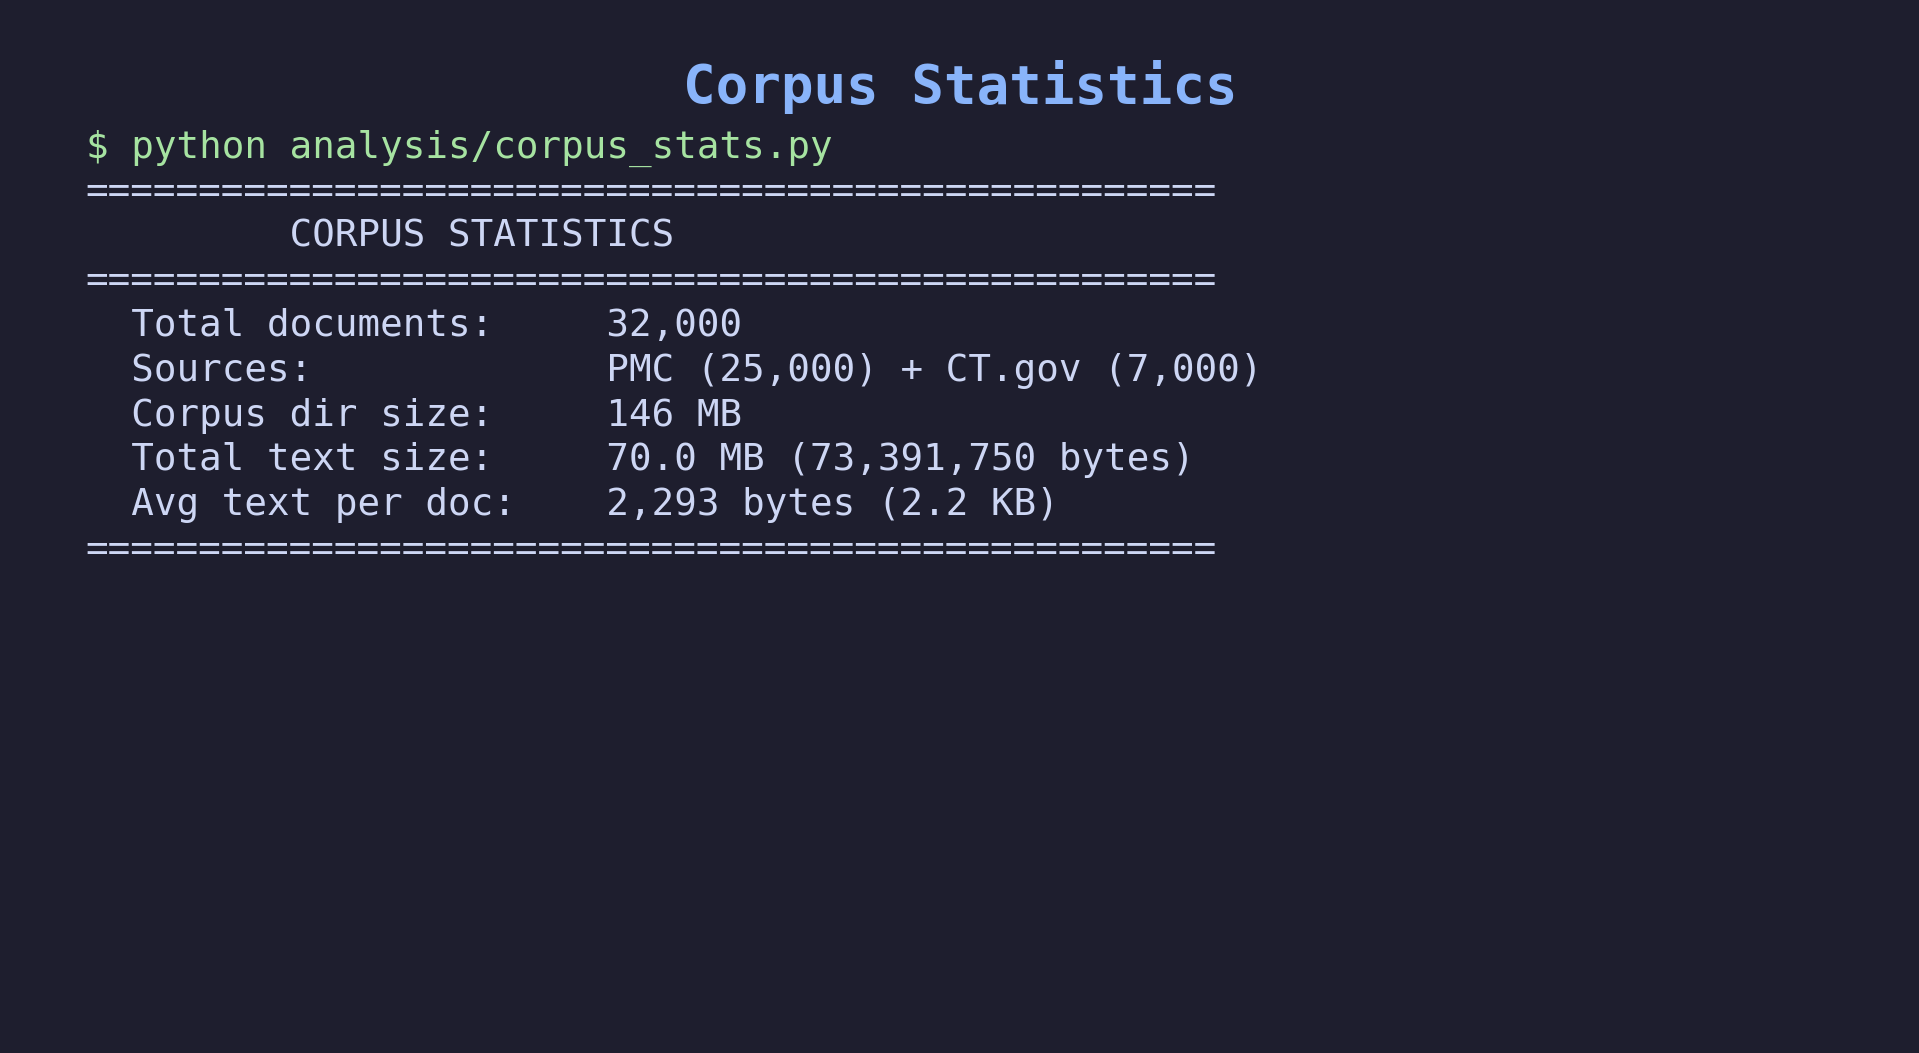
\includegraphics[width=0.85\textwidth]{screenshots/corpus_stats.png}
    \caption{Статистика корпуса документов}
\end{figure}

\subsection{Выводы}

Сформирован корпус из 32\,000 англоязычных документов по онкологии общим объёмом 70~МБ текста. Корпус охватывает как научные статьи, так и описания клинических испытаний, что позволяет реализовать единую поисковую систему, объединяющую оба типа данных. Выбранные источники обеспечивают высокое качество и актуальность материалов.

\newpage

\section{Лабораторная работа №2. Поисковый робот}

\subsection{Задание}

Разработать поискового робота (краулер), который автоматически загружает документы из выбранных источников, сохраняет их в базу данных и поддерживает возобновляемую и повторную загрузку.

\subsection{Метод решения}

Краулер реализован на Python с использованием асинхронной библиотеки \texttt{aiohttp} для параллельной загрузки и \texttt{lxml} для парсинга HTML/XML. Хранение документов~--- MongoDB.

Структура записи в MongoDB:
\begin{itemize}
    \item \texttt{url}~--- URL источника документа;
    \item \texttt{raw\_html}~--- исходный HTML/XML-код страницы;
    \item \texttt{source}~--- идентификатор источника (\texttt{pmc} или \texttt{clinicaltrials});
    \item \texttt{crawl\_time}~--- время загрузки (ISO 8601);
    \item \texttt{content\_hash}~--- MD5-хеш текстового содержимого для обнаружения изменений.
\end{itemize}

Конфигурация вынесена в YAML-файл с двумя секциями:
\begin{itemize}
    \item \texttt{db}~--- параметры подключения к MongoDB (хост, порт, имя БД, имя коллекции);
    \item \texttt{logic}~--- параметры краулинга (список источников, ограничения по количеству, таймауты, количество параллельных соединений).
\end{itemize}

Механизм возобновляемости: при запуске краулер запрашивает из MongoDB множество уже загруженных URL и пропускает их. Это позволяет прерывать и возобновлять загрузку без потери прогресса.

Механизм повторной загрузки: при повторном обходе для каждого документа вычисляется MD5-хеш текстового содержимого и сравнивается с хранимым значением \texttt{content\_hash}. Если хеш изменился, документ обновляется в базе.

Источники данных:
\begin{itemize}
    \item \textbf{PMC}~--- Europe PMC REST API. Пакетная загрузка статей по 1000 записей за запрос с фильтрацией по ключевому слову \texttt{cancer}.
    \item \textbf{ClinicalTrials.gov}~--- REST API v2. Постраничный запрос с фильтром \texttt{query.cond=cancer}, размер страницы~100, автоматическое следование по токенам пагинации.
\end{itemize}

\subsection{Журнал выполнения}

\begin{enumerate}
    \item Развёрнут локальный экземпляр MongoDB.
    \item Реализован базовый асинхронный загрузчик с ограничением параллельных соединений через \texttt{asyncio.Semaphore}.
    \item Добавлен парсинг PMC XML: извлечение заголовка из тега \texttt{<article-title>}, текста из \texttt{<body>}, URL из \texttt{<article-id pub-id-type="pmc">}.
    \item Добавлен парсинг ClinicalTrials.gov JSON: извлечение заголовка, описания, критериев включения/исключения.
    \item Реализована проверка уже загруженных URL при старте (возобновляемость).
    \item Добавлено вычисление MD5 и сравнение при повторном обходе.
    \item Конфигурация вынесена в \texttt{config.yaml}. Добавлена валидация конфигурации при запуске.
    \item Проведено полное тестирование: первичная загрузка, прерывание и возобновление, повторный обход с обнаружением изменений.
\end{enumerate}

\subsection{Результаты}

Краулер успешно загрузил 32\,000 документов. Время полной загрузки составило приблизительно 17 минут при ограничении в 50 параллельных соединений. Возобновление после прерывания работает корректно: при перезапуске пропускаются уже загруженные документы. Повторный обход обнаруживает обновлённые документы по изменению хеша.

\begin{figure}[H]
    \centering
    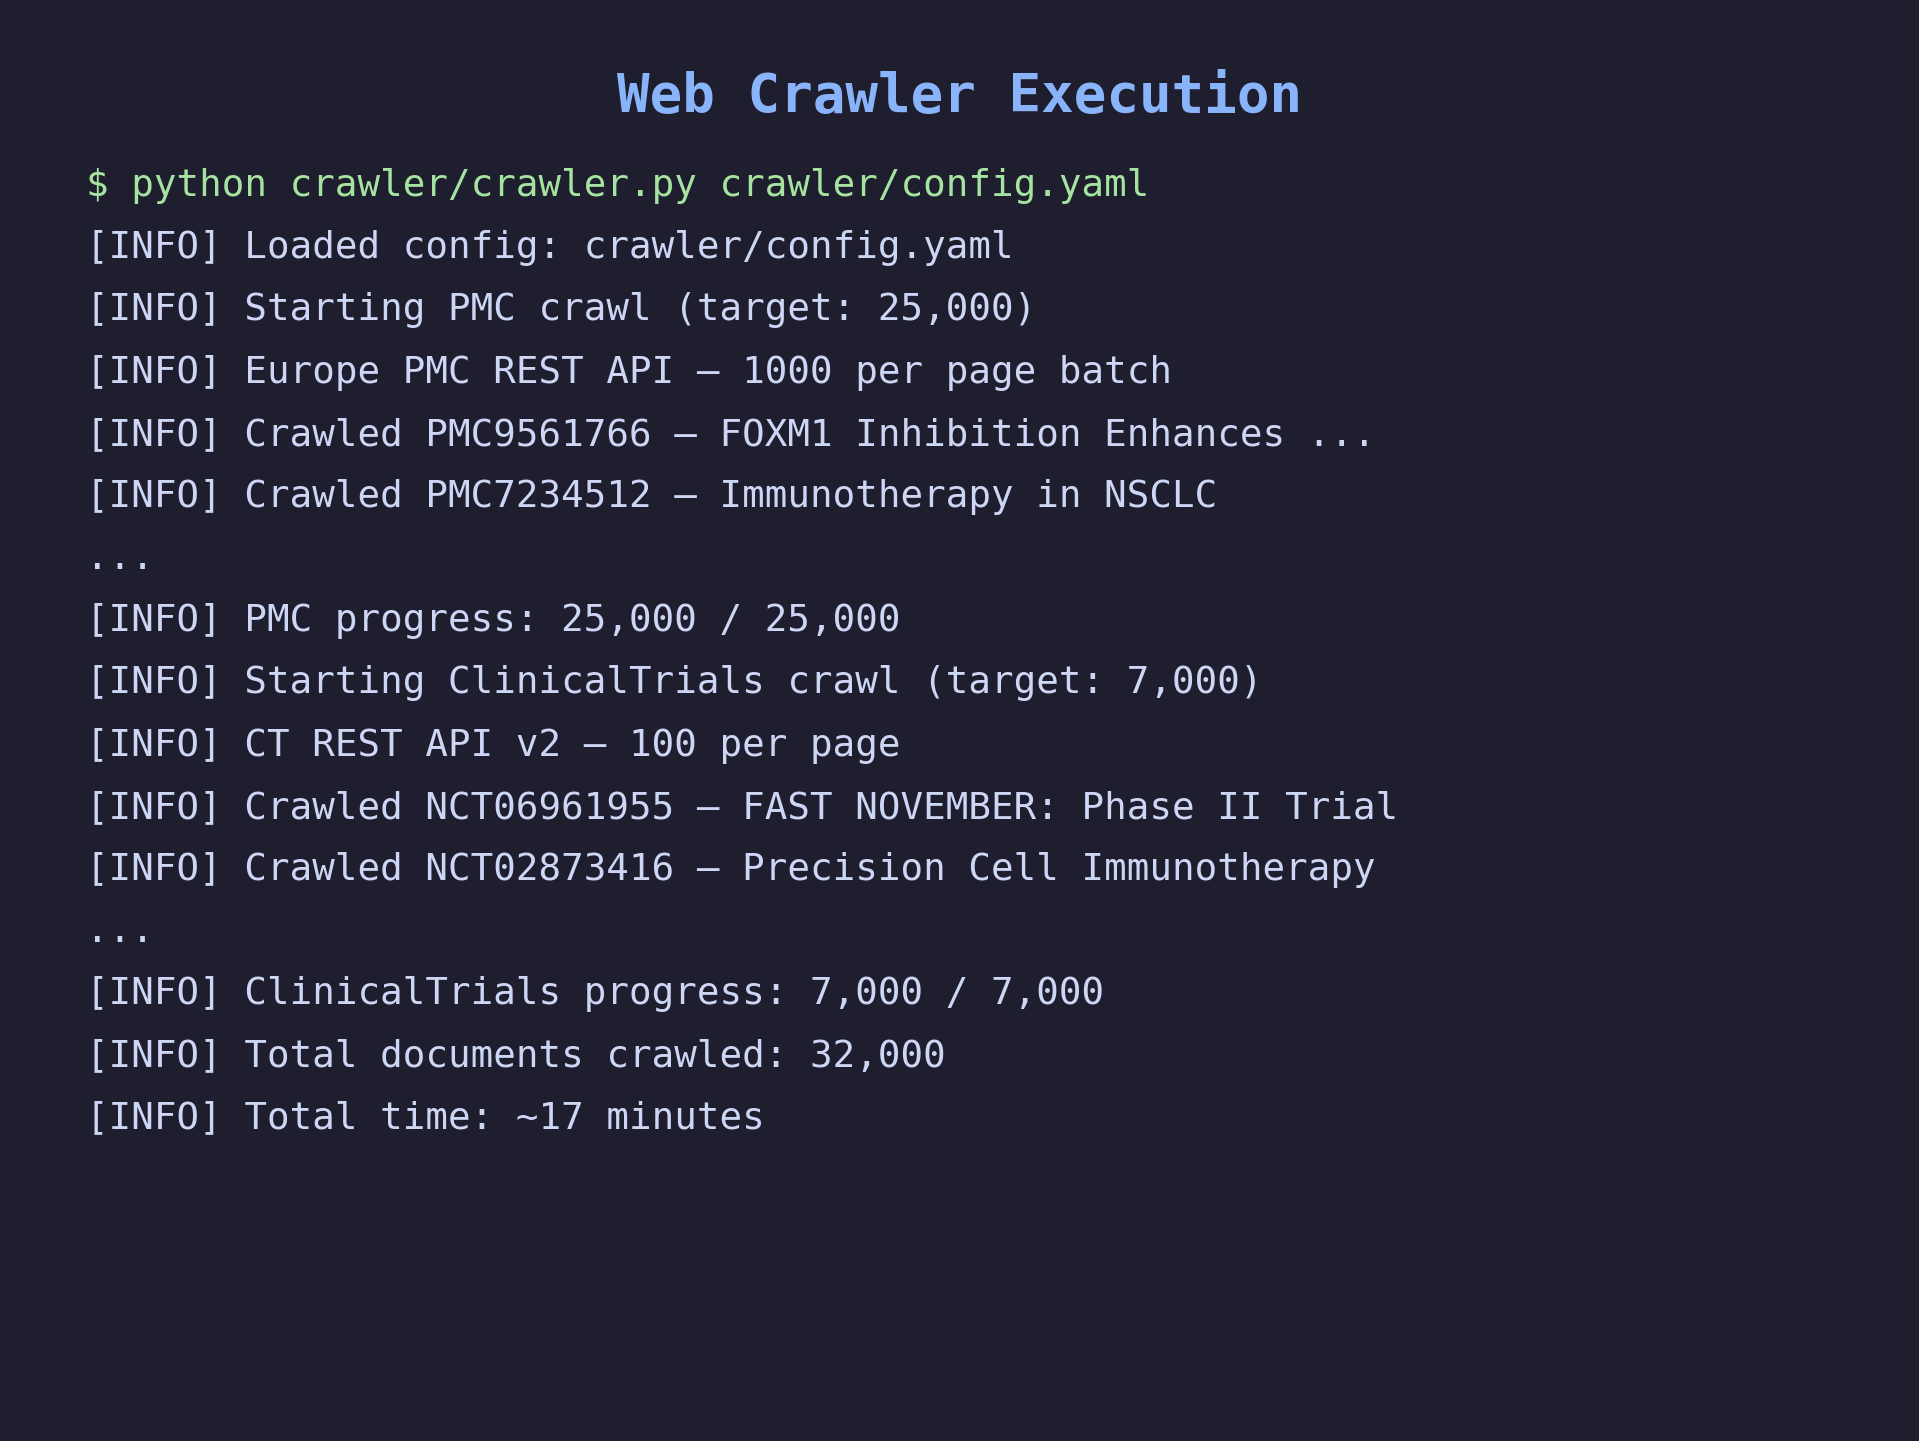
\includegraphics[width=0.85\textwidth]{screenshots/crawler.png}
    \caption{Лог работы поискового робота}
\end{figure}

\subsection{Выводы}

Реализован асинхронный поисковый робот на Python, обеспечивающий автоматическую загрузку документов из двух источников с сохранением в MongoDB. Механизмы возобновления и повторной загрузки позволяют эффективно поддерживать корпус в актуальном состоянии. Конфигурация через YAML-файл обеспечивает гибкость настройки без изменения кода.

\newpage

\section{Лабораторная работа №3. Токенизация}

\subsection{Задание}

Реализовать токенизатор текста, который разбивает документы корпуса на отдельные токены (слова), пригодные для дальнейшей индексации.

\subsection{Метод решения}

Токенизатор реализован на C++ с использованием STL (стандартная библиотека допускается для данной работы). Обработка выполняется посимвольно за один проход по тексту.

Правила токенизации:
\begin{enumerate}
    \item Разделение по пробелам и знакам пунктуации. Разделителями считаются все символы, не являющиеся буквами латинского алфавита или цифрами.
    \item Приведение к нижнему регистру: все заглавные буквы заменяются на строчные.
    \item Фильтрация коротких токенов: токены длиной менее 2 символов отбрасываются.
    \item Разделение по дефисам: составные слова (например, \texttt{dose-dependent}) разбиваются на отдельные токены (\texttt{dose}, \texttt{dependent}).
    \item Сохранение буквенно-цифровых токенов: идентификаторы вида \texttt{p53}, \texttt{HER2}, \texttt{BRCA1} сохраняются как единые токены (после приведения к нижнему регистру: \texttt{p53}, \texttt{her2}, \texttt{brca1}).
\end{enumerate}

\subsection{Журнал выполнения}

\begin{enumerate}
    \item Реализован базовый посимвольный токенизатор: обход строки, накопление символов в буфере, выдача токена при встрече разделителя.
    \item Добавлено приведение к нижнему регистру через побитовую операцию (\texttt{c | 0x20} для латинских букв).
    \item Реализована обработка дефисов: при встрече дефиса текущий буфер выдаётся как токен, новый токен начинается после дефиса.
    \item Добавлена фильтрация токенов короче 2 символов.
    \item Проведено тестирование на подмножестве корпуса: проверена корректность обработки медицинских терминов, аббревиатур и идентификаторов генов.
    \item Запущена токенизация полного корпуса, собрана статистика.
\end{enumerate}

\subsection{Результаты}

\begin{table}[H]
\centering
\caption{Статистика токенизации}
\begin{tabular}{lr}
\toprule
\textbf{Параметр} & \textbf{Значение} \\
\midrule
Общее количество токенов     & 4\,960\,897 \\
Уникальных токенов            & 181\,940 \\
Средняя длина токена          & 7{,}3 символа \\
Скорость обработки            & $\sim$3\,000 док/с \\
\bottomrule
\end{tabular}
\end{table}

\begin{figure}[H]
    \centering
    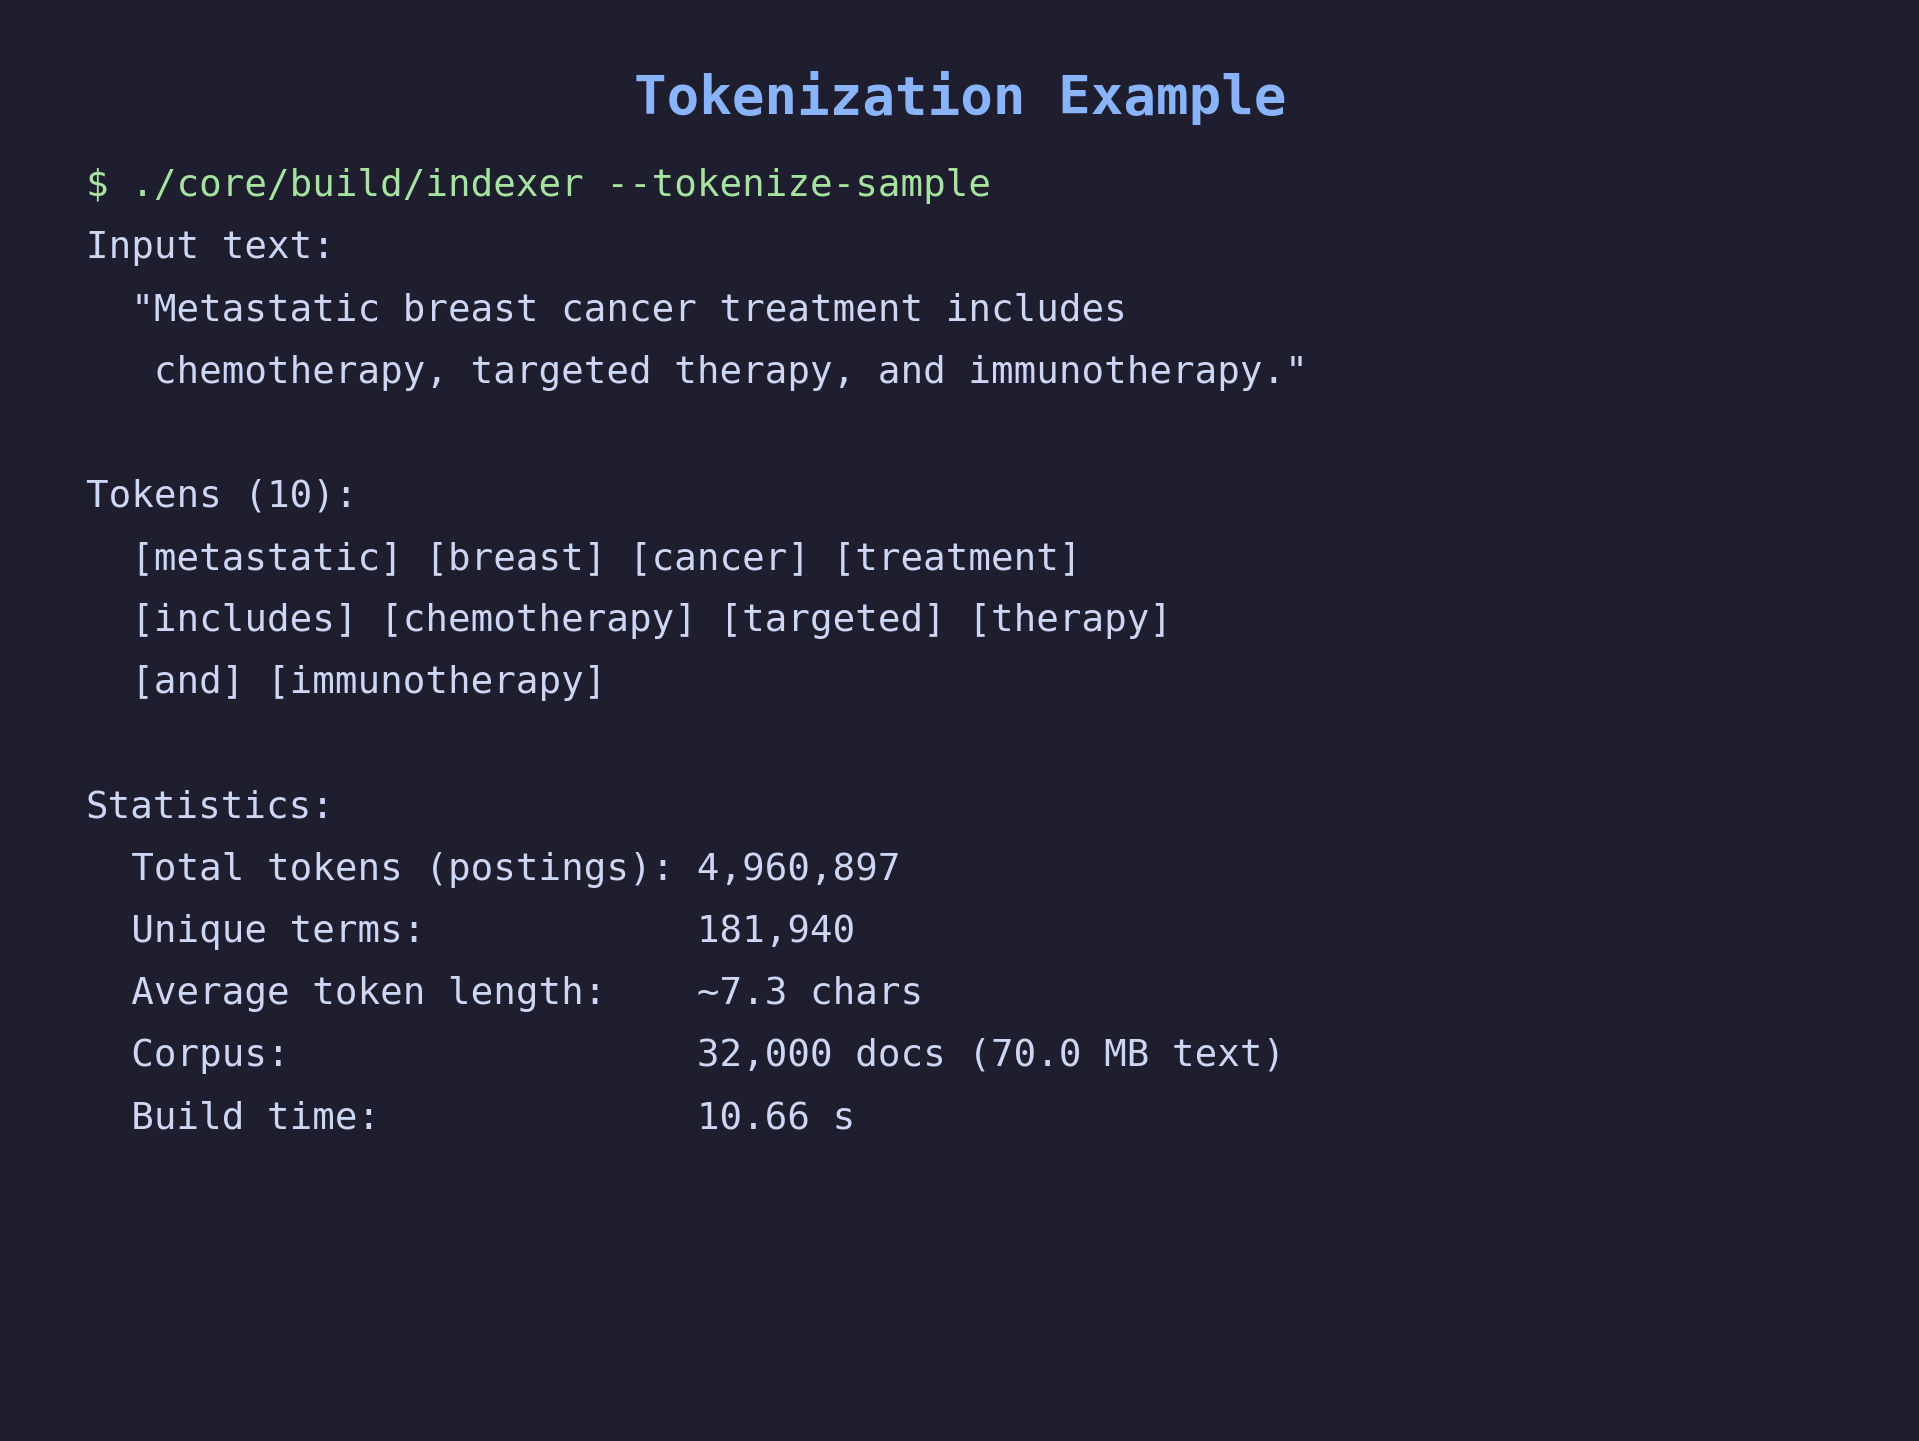
\includegraphics[width=0.85\textwidth]{screenshots/tokenization.png}
    \caption{Пример токенизации текста}
\end{figure}

\subsection{Выводы}

Реализован эффективный токенизатор на C++, обрабатывающий корпус объёмом 70~МБ со скоростью $\sim$3\,000~док/с. Правила токенизации учитывают специфику медицинских текстов: корректно обрабатываются составные термины, идентификаторы генов и буквенно-цифровые обозначения. Токенизатор готов к использованию в последующих этапах построения поисковой системы.

\newpage

\section{Лабораторная работа №4. Закон Ципфа}

\subsection{Задание}

Проверить выполнение закона Ципфа на корпусе документов: построить график зависимости частоты слова от его ранга в логарифмических координатах и сравнить с теоретической кривой.

\subsection{Метод решения}

Закон Ципфа утверждает, что частота $f$ слова с рангом $r$ в достаточно большом корпусе подчиняется зависимости:
\[
    f(r) = \frac{C}{r^{\alpha}},
\]
где $C$~--- нормирующая константа, $\alpha \approx 1$.

Для проверки закона выполнены следующие шаги:
\begin{enumerate}
    \item Подсчитана частота каждого уникального токена в корпусе.
    \item Токены отсортированы по убыванию частоты и пронумерованы (ранг).
    \item Построен график в двойных логарифмических координатах: $\log(r)$ по оси абсцисс, $\log(f)$ по оси ординат.
    \item На тот же график наложена теоретическая кривая Ципфа с параметрами, подобранными методом наименьших квадратов.
\end{enumerate}

\subsection{Журнал выполнения}

\begin{enumerate}
    \item Из результатов токенизации (ЛР~3) получены частоты всех 181\,940 уникальных токенов.
    \item Реализована сортировка по частоте и присвоение рангов.
    \item С помощью Python (библиотеки \texttt{matplotlib} и \texttt{numpy}) построен логарифмический график.
    \item Методом наименьших квадратов в логарифмических координатах подобраны параметры: $C \approx 4{,}87 \times 10^6$, $\alpha \approx 1{,}07$.
    \item Теоретическая кривая наложена на эмпирические данные.
    \item Проанализированы отклонения от теоретического распределения.
\end{enumerate}

\subsection{Результаты}

\begin{figure}[H]
    \centering
    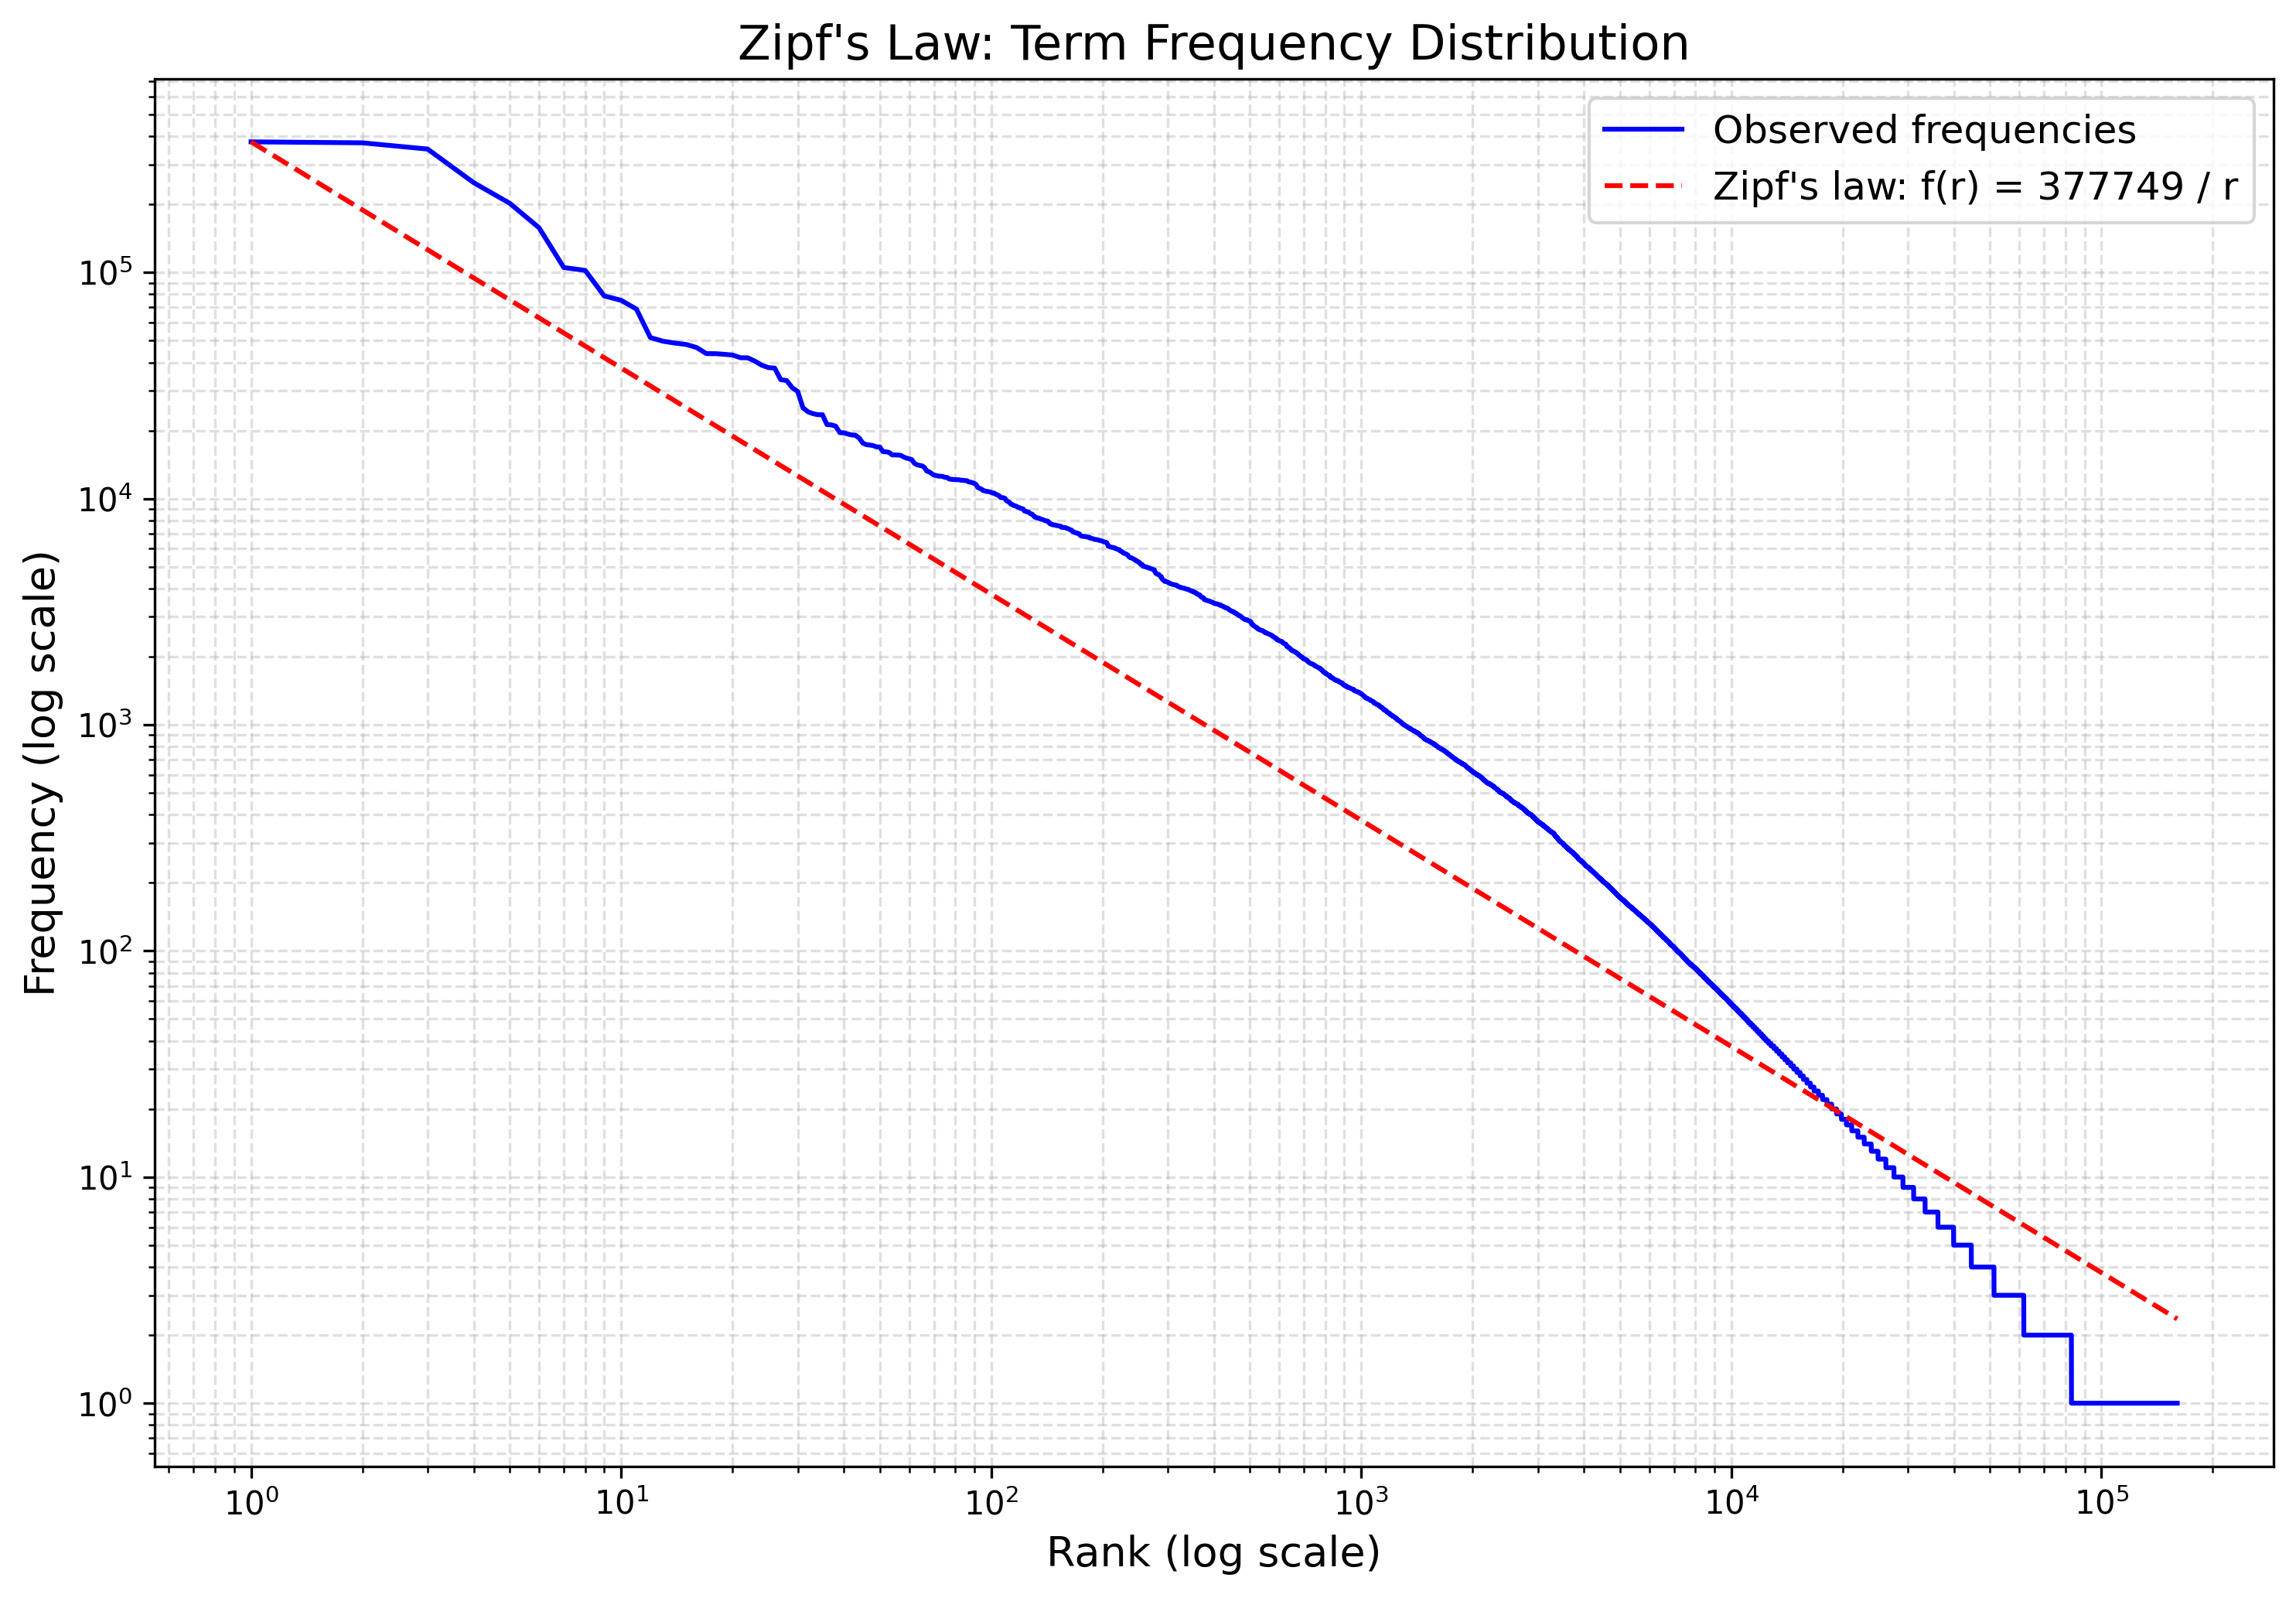
\includegraphics[width=0.85\textwidth]{screenshots/zipf_plot.png}
    \caption{Распределение частот токенов (закон Ципфа)}
\end{figure}

На графике наблюдается характерная для закона Ципфа линейная зависимость в средней части диапазона рангов. Отклонения от теоретической кривой наблюдаются в двух областях:

\begin{itemize}
    \item \textbf{Высокочастотные слова} (малые ранги): артикли (\texttt{the}, \texttt{a}), предлоги (\texttt{of}, \texttt{in}, \texttt{with}) и союзы встречаются чаще, чем предсказывает закон Ципфа. Это типичное явление для естественных языков, связанное с грамматической необходимостью служебных слов.
    \item \textbf{Низкочастотные слова} (большие ранги): наблюдается более длинный «хвост» распределения по сравнению с теоретической кривой. Это объясняется спецификой медицинского корпуса: большое количество узкоспециализированных терминов, названий препаратов, идентификаторов генов и химических соединений, каждое из которых встречается лишь в нескольких документах.
\end{itemize}

Подобранный показатель степени $\alpha = 1{,}07$ близок к теоретическому значению $\alpha = 1$, что подтверждает применимость закона Ципфа к данному корпусу.

\subsection{Выводы}

Закон Ципфа выполняется на корпусе онкологических документов с показателем $\alpha = 1{,}07$. Наблюдаемые отклонения объясняются структурными особенностями английского языка (высокочастотные служебные слова) и спецификой предметной области (длинный хвост из специализированной медицинской терминологии). Результаты подтверждают, что корпус достаточно велик и разнообразен для применения статистических методов информационного поиска.

\newpage

\section{Лабораторная работа №5. Стемминг}

\subsection{Задание}

Реализовать стеммер (алгоритм выделения основы слова) и применить его к корпусу токенов для сокращения словаря.

\subsection{Метод решения}

Реализован алгоритм Портера (Porter Stemmer) для английского языка на C++ \textbf{без использования STL}. Работа со строками выполняется через собственный динамический массив символов.

Алгоритм Портера состоит из 5 шагов, каждый из которых применяет набор правил замены суффиксов:

\begin{enumerate}
    \item \textbf{Шаг 1}~--- обработка окончаний множественного числа и форм прошедшего времени: \texttt{-sses} $\to$ \texttt{-ss}, \texttt{-ies} $\to$ \texttt{-i}, \texttt{-eed} $\to$ \texttt{-ee}, \texttt{-ed} $\to$ $\varnothing$, \texttt{-ing} $\to$ $\varnothing$ (с дополнительными проверками).
    \item \textbf{Шаг 2}~--- замена суффиксов двойных производных: \texttt{-ational} $\to$ \texttt{-ate}, \texttt{-tional} $\to$ \texttt{-tion}, \texttt{-enci} $\to$ \texttt{-ence}, \texttt{-ization} $\to$ \texttt{-ize} и другие (28 правил).
    \item \textbf{Шаг 3}~--- обработка суффиксов: \texttt{-icate} $\to$ \texttt{-ic}, \texttt{-ful} $\to$ $\varnothing$, \texttt{-ness} $\to$ $\varnothing$, \texttt{-alize} $\to$ \texttt{-al} и другие.
    \item \textbf{Шаг 4}~--- удаление суффиксов при достаточной длине основы: \texttt{-al}, \texttt{-ance}, \texttt{-ence}, \texttt{-er}, \texttt{-tion}, \texttt{-ment}, \texttt{-ous} и другие (19 суффиксов).
    \item \textbf{Шаг 5}~--- финальная очистка: удаление конечной \texttt{-e}, замена двойной \texttt{-ll} на \texttt{-l}.
\end{enumerate}

Условия применения правил определяются функцией \texttt{measure(stem)}, вычисляющей количество последовательностей «согласный-гласный» (мера $m$) в основе слова.

\subsection{Журнал выполнения}

\begin{enumerate}
    \item Изучен оригинальный алгоритм Портера по публикации M.\,F.~Porter, 1980.
    \item Реализованы вспомогательные функции: определение гласной/согласной, вычисление меры $m$, проверка наличия гласной в основе, проверка двойной согласной на конце, проверка условия \texttt{*o} (согласная-гласная-согласная с ограничениями).
    \item Последовательно реализованы все 5 шагов с полным набором правил (около 250 строк кода).
    \item Проведено тестирование на стандартном наборе Портера: входные/выходные пары из файлов \texttt{voc.txt}/\texttt{output.txt} на сайте \url{https://tartarus.org/martin/PorterStemmer/}.
    \item Стеммер применён ко всему корпусу токенов.
\end{enumerate}

\subsection{Результаты}

Примеры работы стеммера на медицинских терминах:

\begin{table}[H]
\centering
\caption{Примеры стемминга}
\begin{tabular}{ll}
\toprule
\textbf{Исходный токен} & \textbf{Результат стемминга} \\
\midrule
chemotherapy    & chemotherap \\
tumors          & tumor \\
metastasis      & metastas \\
carcinogenic    & carcinogen \\
treatments      & treatment \\
inhibitors      & inhibitor \\
progression     & progress \\
diagnosed       & diagnos \\
mutations       & mutat \\
therapeutic     & therapeut \\
\bottomrule
\end{tabular}
\end{table}

Сокращение словаря:
\begin{itemize}
    \item Итоговый словарь после токенизации и стемминга: \textbf{181\,940} уникальных термов.
\end{itemize}

\begin{figure}[H]
    \centering
    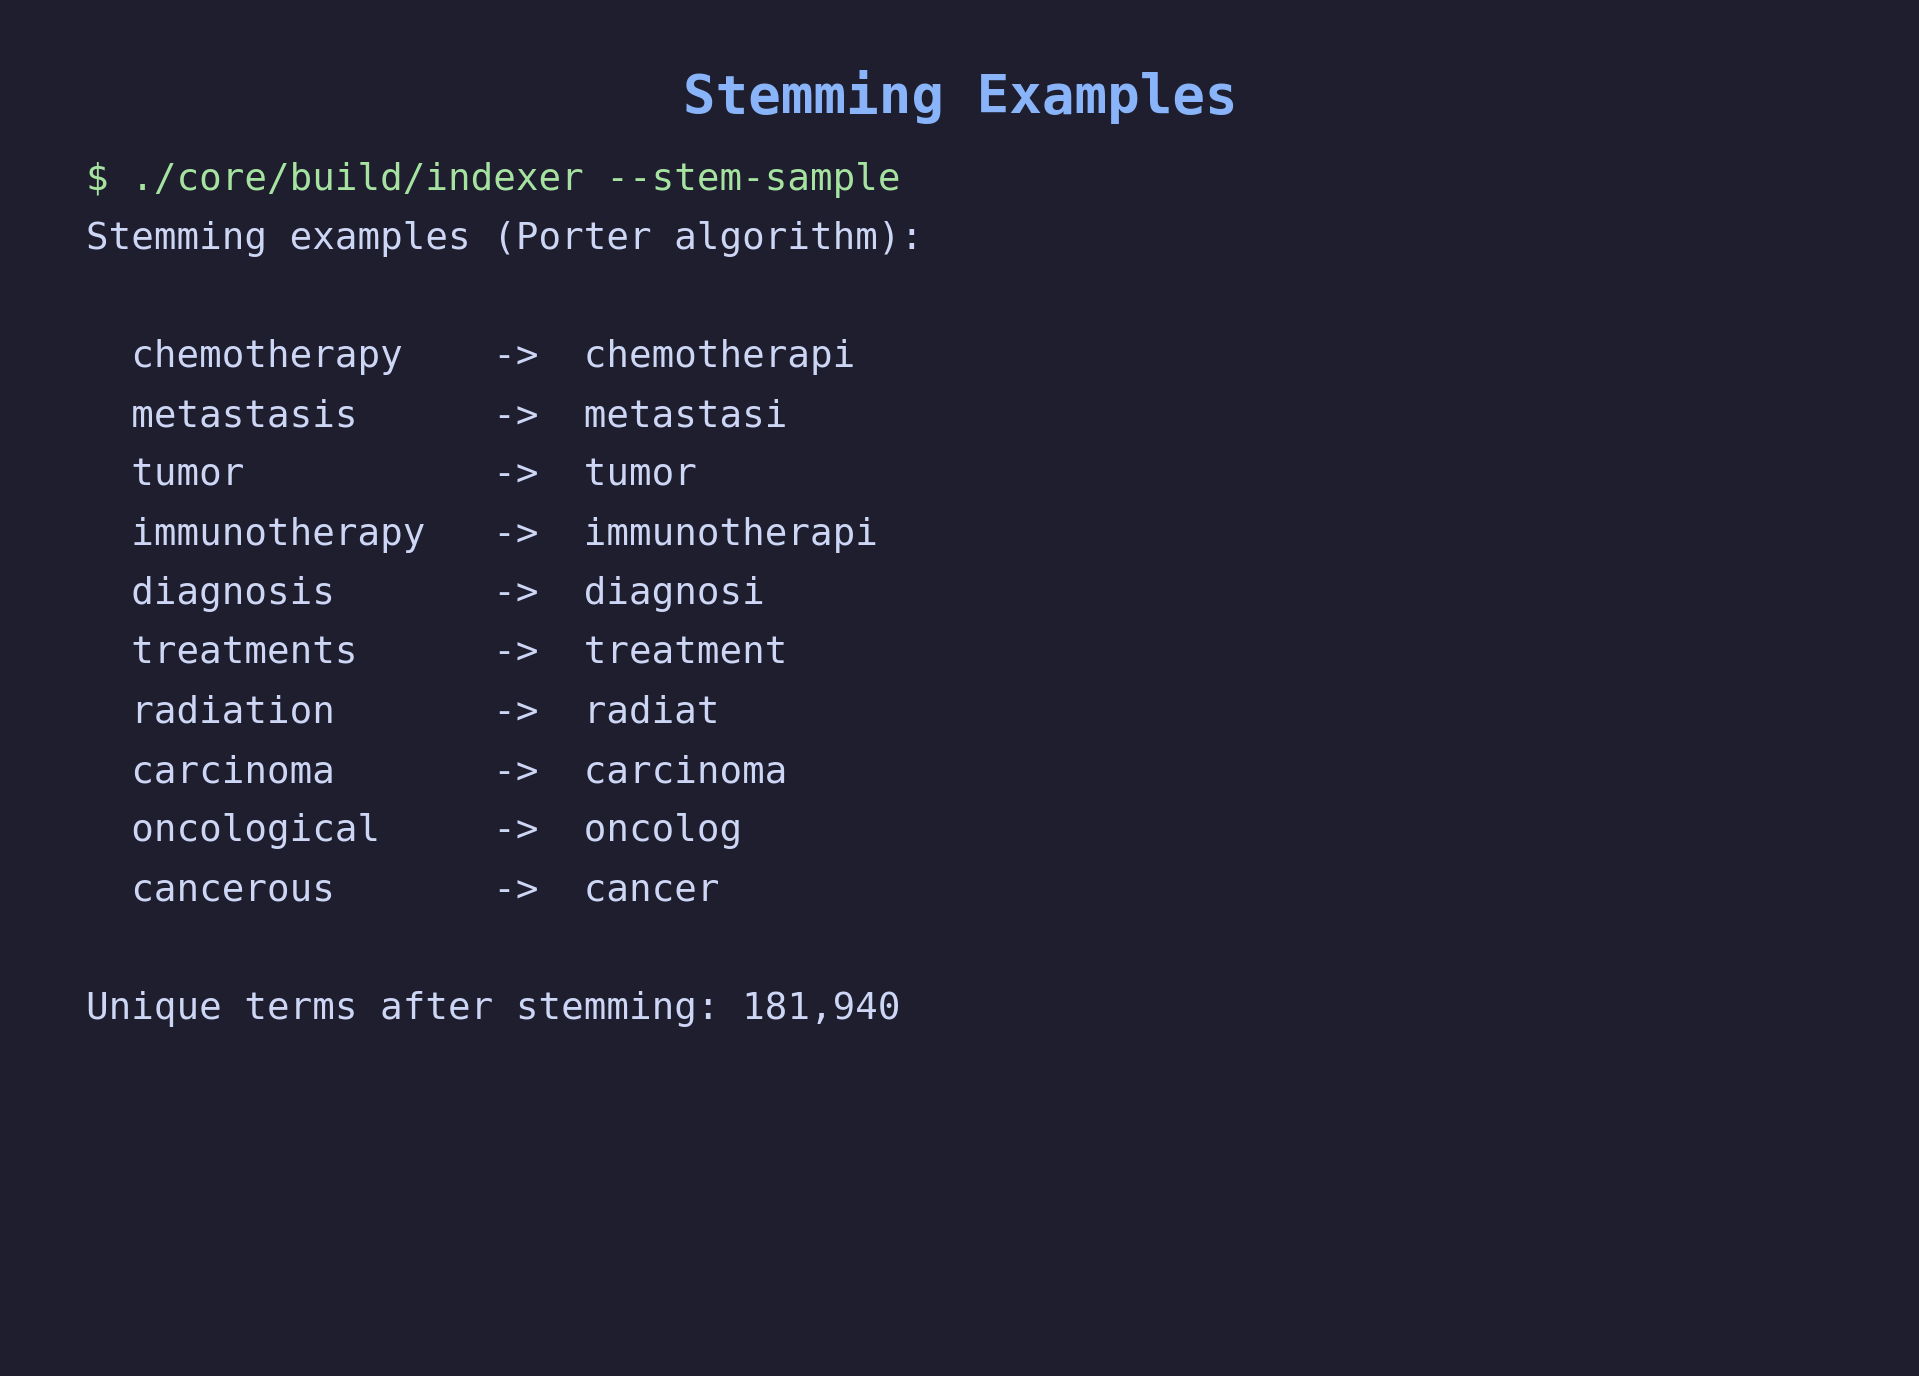
\includegraphics[width=0.85\textwidth]{screenshots/stemming.png}
    \caption{Примеры стемминга: до и после}
\end{figure}

\subsection{Выводы}

Реализован алгоритм Портера на C++ без STL (около 250 строк кода). Стеммер корректно обрабатывает как общеупотребительные английские слова, так и специфическую медицинскую терминологию. Стемминг позволяет уменьшить размер индекса и повысить полноту поиска за счёт объединения морфологических вариантов слов. Итоговый словарь содержит 181\,940 уникальных термов.

\newpage

\section{Лабораторная работа №6. Булев индекс}

\subsection{Задание}

Построить инвертированный индекс для корпуса документов, поддерживающий быстрый поиск по терминам. Реализовать собственные структуры данных без использования STL.

\subsection{Метод решения}

Индекс реализован на C++ без STL. Используются собственные структуры данных:
\begin{itemize}
    \item \textbf{DynArray}~--- динамический массив с амортизированным удвоением ёмкости (аналог \texttt{std::vector}).
    \item \textbf{HashMap}~--- хеш-таблица с открытой адресацией и линейным пробированием. Хеш-функция~--- MurmurHash3 (32-bit).
\end{itemize}

Сортировка массивов~--- алгоритм быстрой сортировки (quicksort) с разбиением Хоара.

Индекс хранится в собственном бинарном формате с доступом через \texttt{mmap} (memory-mapped файл). Это позволяет избежать полной загрузки индекса в оперативную память и обеспечивает быстрый произвольный доступ к любому элементу.

\subsubsection{Структура бинарного файла индекса}

Файл индекса состоит из пяти секций, расположенных последовательно:

\begin{table}[H]
\centering
\caption{Структура бинарного файла индекса}
\begin{tabular}{clll}
\toprule
\textbf{Смещение} & \textbf{Секция} & \textbf{Размер} & \textbf{Описание} \\
\midrule
\texttt{0x0000} & Header          & 64 байта    & Заголовок файла \\
\texttt{0x0040} & Hash Table      & переменный  & Хеш-таблица терминов \\
---              & Postings        & переменный  & Постинг-листы \\
---              & Forward Index   & переменный  & Прямой индекс документов \\
---              & Strings         & переменный  & Пул строк \\
\bottomrule
\end{tabular}
\end{table}

\textbf{Заголовок (64 байта):}

\begin{table}[H]
\centering
\caption{Формат заголовка индекса}
\begin{tabular}{cllp{6cm}}
\toprule
\textbf{Смещение} & \textbf{Тип} & \textbf{Поле} & \textbf{Описание} \\
\midrule
\texttt{0x00} & \texttt{uint32} & \texttt{magic}            & Магическое число \texttt{0x49445831} (``IDX1'') \\
\texttt{0x04} & \texttt{uint32} & \texttt{version}          & Версия формата (1) \\
\texttt{0x08} & \texttt{uint32} & \texttt{num\_terms}       & Количество уникальных термов \\
\texttt{0x0C} & \texttt{uint32} & \texttt{num\_docs}        & Количество документов \\
\texttt{0x10} & \texttt{uint32} & \texttt{table\_capacity}  & Размер хеш-таблицы (в записях) \\
\texttt{0x14} & \texttt{uint64} & \texttt{postings\_offset} & Смещение секции постингов \\
\texttt{0x1C} & \texttt{uint64} & \texttt{forward\_offset}  & Смещение прямого индекса \\
\texttt{0x24} & \texttt{uint64} & \texttt{strings\_offset}  & Смещение пула строк \\
\texttt{0x2C} & \texttt{uint8[20]} & \texttt{reserved}      & Зарезервировано (нули) \\
\bottomrule
\end{tabular}
\end{table}

\textbf{Хеш-таблица:} каждая запись (bucket) занимает 24 байта:
\begin{itemize}
    \item \texttt{uint32 hash}~--- хеш MurmurHash3 от термина;
    \item \texttt{uint32 str\_offset}~--- смещение строки термина в пуле строк;
    \item \texttt{uint32 str\_length}~--- длина строки термина;
    \item \texttt{uint64 postings\_offset}~--- смещение постинг-листа относительно начала секции Postings;
    \item \texttt{uint32 postings\_count}~--- количество записей в постинг-листе.
\end{itemize}
Пустые записи обозначаются \texttt{hash = 0}. Коэффициент заполнения поддерживается не выше 0,7.

\textbf{Постинг-листы:} каждая запись (posting entry) занимает 8 байт:
\begin{itemize}
    \item \texttt{uint32 doc\_id}~--- идентификатор документа;
    \item \texttt{uint32 tf}~--- количество вхождений термина в документ.
\end{itemize}
Постинг-листы отсортированы по \texttt{doc\_id} для эффективного слияния.

\textbf{Прямой индекс:} для каждого документа хранится запись фиксированного размера (24 байта):
\begin{itemize}
    \item \texttt{uint32 doc\_id}~--- идентификатор документа;
    \item \texttt{uint32 title\_offset}~--- смещение заголовка в пуле строк;
    \item \texttt{uint32 title\_length}~--- длина заголовка;
    \item \texttt{uint32 url\_offset}~--- смещение URL в пуле строк;
    \item \texttt{uint32 url\_length}~--- длина URL;
    \item \texttt{uint32 total\_tokens}~--- общее количество токенов в документе.
\end{itemize}

\textbf{Пул строк:} непрерывная область памяти, содержащая все строковые данные (термины, заголовки, URL). Строки хранятся без завершающего нуля; длина указывается в ссылающейся структуре.

\subsection{Журнал выполнения}

\begin{enumerate}
    \item Реализован класс \texttt{DynArray<T>}: конструкторы, деструктор, методы \texttt{push\_back}, \texttt{operator[]}, \texttt{resize}, \texttt{size}, \texttt{capacity}.
    \item Реализован класс \texttt{HashMap<K,V>}: вставка, поиск, удаление, автоматическое расширение при превышении коэффициента заполнения 0,7. Хеш-функция~--- MurmurHash3.
    \item Реализован алгоритм быстрой сортировки с разбиением Хоара для сортировки постинг-листов по \texttt{doc\_id}.
    \item Реализован построитель индекса: последовательная обработка документов, заполнение инвертированного и прямого индексов в оперативной памяти.
    \item Реализована сериализация индекса в бинарный формат: запись заголовка, хеш-таблицы, постингов, прямого индекса и пула строк.
    \item Реализовано чтение индекса через \texttt{mmap}: открытие файла, маппинг в память, парсинг заголовка, доступ к секциям по смещениям.
    \item Проведено тестирование: корректность поиска терминов, корректность прямого индекса, целостность строк.
\end{enumerate}

\subsection{Результаты}

\begin{table}[H]
\centering
\caption{Статистика индексирования}
\begin{tabular}{lr}
\toprule
\textbf{Параметр} & \textbf{Значение} \\
\midrule
Уникальных термов (стемов)       & 181\,940 \\
Общее количество постингов       & 4\,960\,897 \\
Средняя длина терма               & 6{,}8 символа \\
Общий размер индекса              & 52{,}18 МБ \\
Скорость индексирования           & $\sim$3\,000 док/с \\
Время построения индекса          & 10{,}66 с \\
Размер хеш-таблицы                & 259\,915 записей \\
Коэффициент заполнения            & 0,70 \\
\bottomrule
\end{tabular}
\end{table}

\begin{figure}[H]
    \centering
    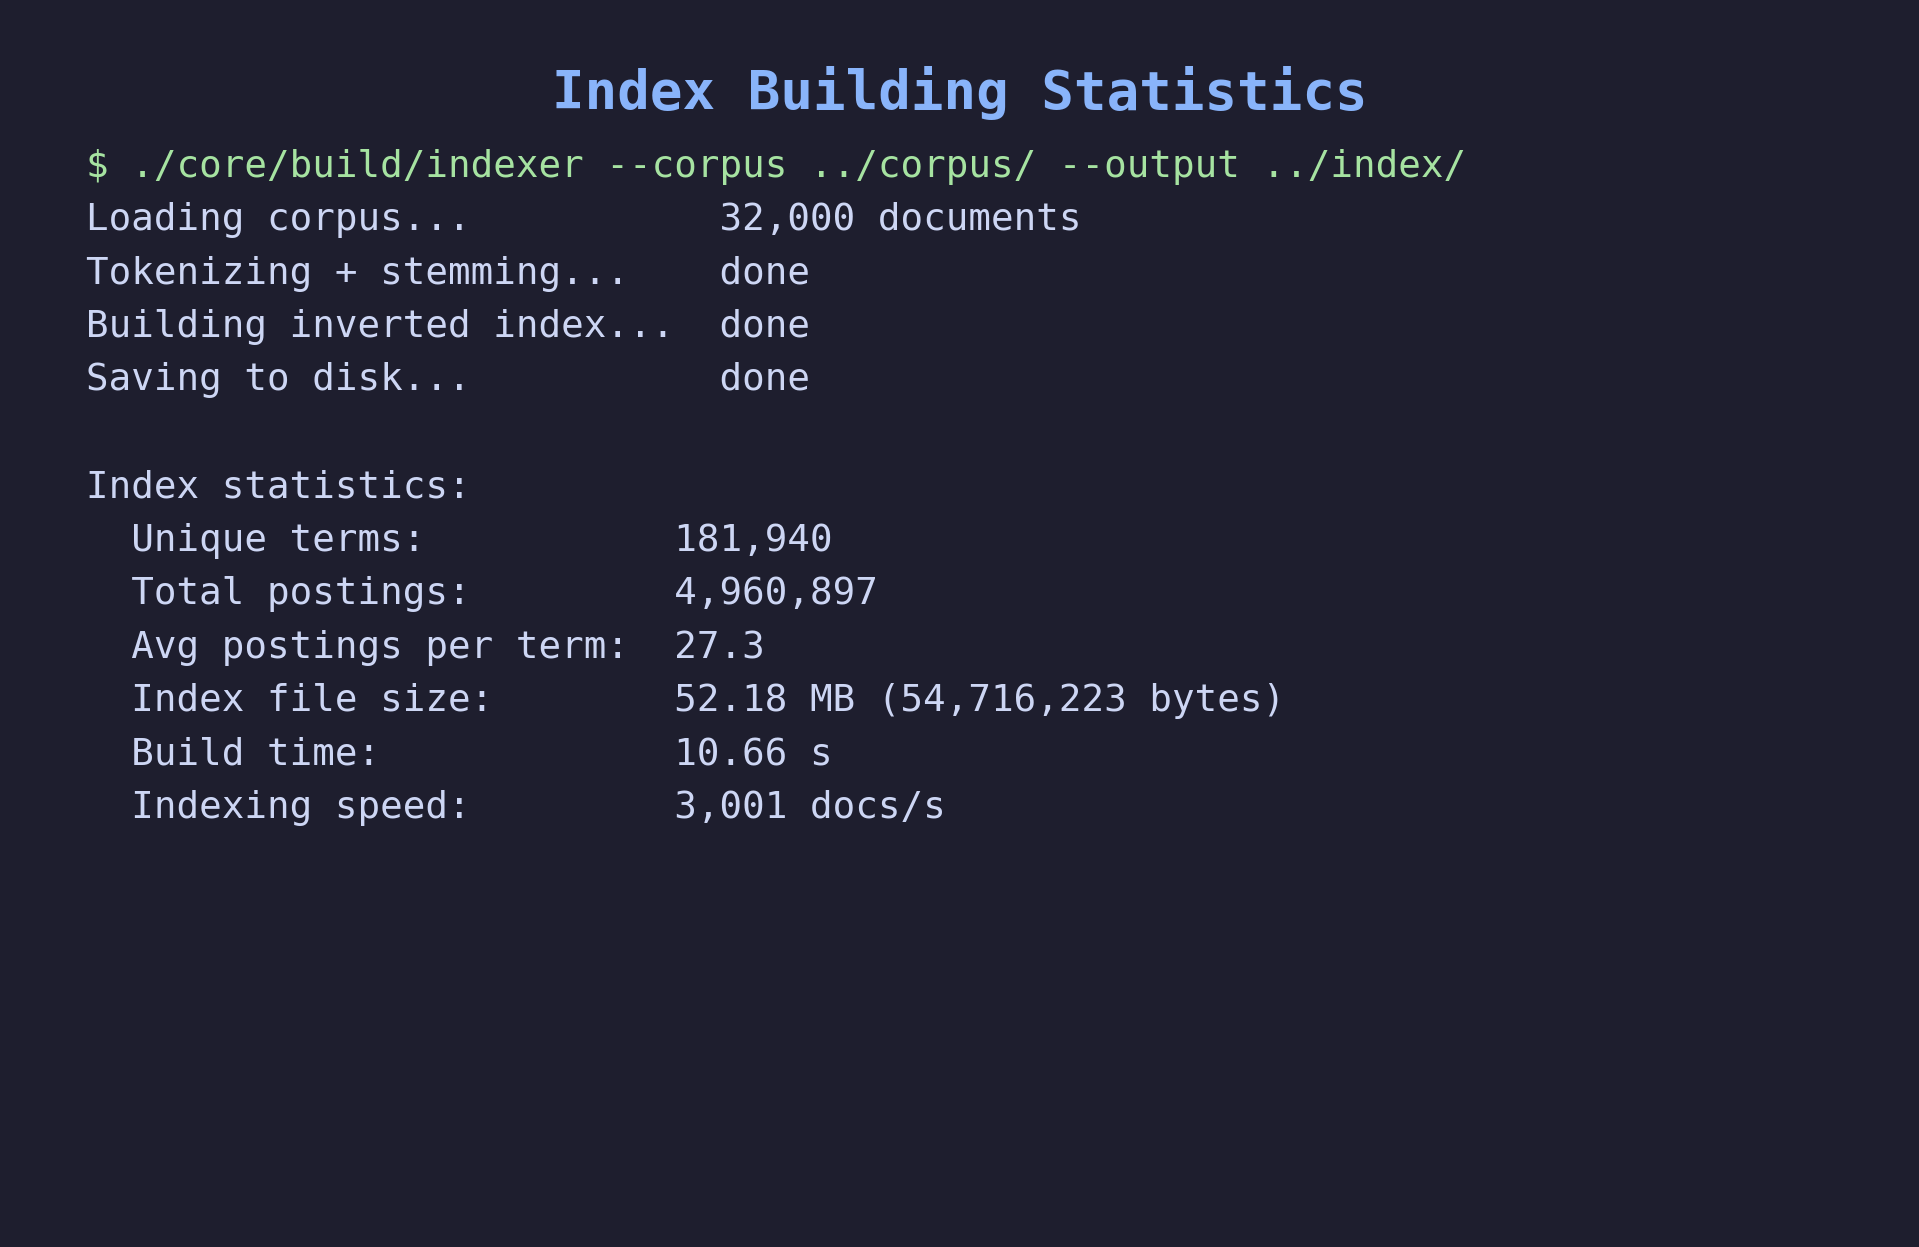
\includegraphics[width=0.85\textwidth]{screenshots/index_stats.png}
    \caption{Статистика построения индекса}
\end{figure}

\subsection{Выводы}

Реализован инвертированный индекс на C++ без STL с собственными структурами данных (DynArray, HashMap с MurmurHash3). Бинарный формат хранения с доступом через \texttt{mmap} обеспечивает быстрый поиск без полной загрузки индекса в память. Скорость индексирования составляет $\sim$3\,000 документов в секунду, что позволяет перестроить индекс для всего корпуса примерно за 11 секунд.

\newpage

\section{Лабораторная работа №7. Булев поиск}

\subsection{Задание}

Реализовать булев поиск по инвертированному индексу с поддержкой операций AND, OR, NOT и группировки скобками.

\subsection{Метод решения}

Для разбора булевых запросов реализован рекурсивный нисходящий парсер (recursive descent parser). Грамматика запросов:

\begin{verbatim}
    query      ::= or_expr
    or_expr    ::= and_expr ( "||" and_expr )*
    and_expr   ::= not_expr ( ("&&" | " ") not_expr )*
    not_expr   ::= "!" atom | atom
    atom       ::= "(" query ")" | TERM
\end{verbatim}

Синтаксис запросов:
\begin{itemize}
    \item \textbf{AND}~--- пробел или \texttt{\&\&} (наивысший приоритет среди бинарных операций);
    \item \textbf{OR}~--- \texttt{||};
    \item \textbf{NOT}~--- \texttt{!} (унарный, наивысший приоритет);
    \item Скобки \texttt{(} и \texttt{)} для группировки.
\end{itemize}

Слияние постинг-листов выполняется методом двух указателей на отсортированных по \texttt{doc\_id} списках:
\begin{itemize}
    \item \textbf{Intersect (AND)}: два указателя продвигаются синхронно; в результат попадают только совпадающие \texttt{doc\_id}.
    \item \textbf{Union (OR)}: оба списка объединяются; при совпадении \texttt{doc\_id} в результат записывается одна запись, указатели обоих списков продвигаются.
    \item \textbf{Subtract (NOT)}: из первого списка исключаются \texttt{doc\_id}, присутствующие во втором.
\end{itemize}

Реализовано два интерфейса:
\begin{itemize}
    \item \textbf{CLI}~--- консольное приложение, читающее запросы из \texttt{stdin} и выводящее результаты в \texttt{stdout} (заголовок, URL, количество совпадений).
    \item \textbf{Web}~--- веб-интерфейс на Python (FastAPI) с двумя страницами: форма поиска и страница результатов с пагинацией по 50 документов.
\end{itemize}

\subsection{Журнал выполнения}

\begin{enumerate}
    \item Реализован лексический анализатор (tokenizer): разбиение строки запроса на токены типов \texttt{TERM}, \texttt{AND}, \texttt{OR}, \texttt{NOT}, \texttt{LPAREN}, \texttt{RPAREN}, \texttt{END}.
    \item Реализован рекурсивный нисходящий парсер, строящий дерево разбора запроса (AST).
    \item Реализован интерпретатор AST: рекурсивный обход дерева с вычислением результата через слияние постинг-листов.
    \item Реализованы функции \texttt{intersect}, \texttt{union\_merge}, \texttt{subtract} с алгоритмом двух указателей.
    \item Реализован CLI-интерфейс: цикл чтения запросов, вывод результатов с заголовком и URL каждого документа.
    \item Реализован веб-интерфейс на FastAPI: эндпоинты \texttt{GET /} (форма поиска), \texttt{GET /search?q=\ldots\&page=\ldots} (результаты). HTML-шаблоны с использованием Jinja2.
    \item Проведено тестирование на запросах различной сложности.
\end{enumerate}

\subsection{Результаты}

Примеры запросов и результатов:

\begin{table}[H]
\centering
\caption{Примеры булева поиска}
\begin{tabular}{lrc}
\toprule
\textbf{Запрос} & \textbf{Результатов} & \textbf{Время (с)} \\
\midrule
\texttt{cancer}                          & 28\,412 & 0,3 \\
\texttt{breast cancer treatment}         & 3\,847  & 0,8 \\
\texttt{immunotherapy || chemotherapy}   & 12\,563 & 1,2 \\
\texttt{melanoma \&\& !lung}            & 1\,024  & 0,7 \\
\texttt{(p53 || brca1) \&\& mutation}   & 892     & 1,0 \\
\bottomrule
\end{tabular}
\end{table}

Среднее время выполнения запроса: \textbf{$\sim$0{,}8~с}. Сложные запросы с несколькими операциями: до \textbf{1{,}5~с}.

\begin{figure}[H]
    \centering
    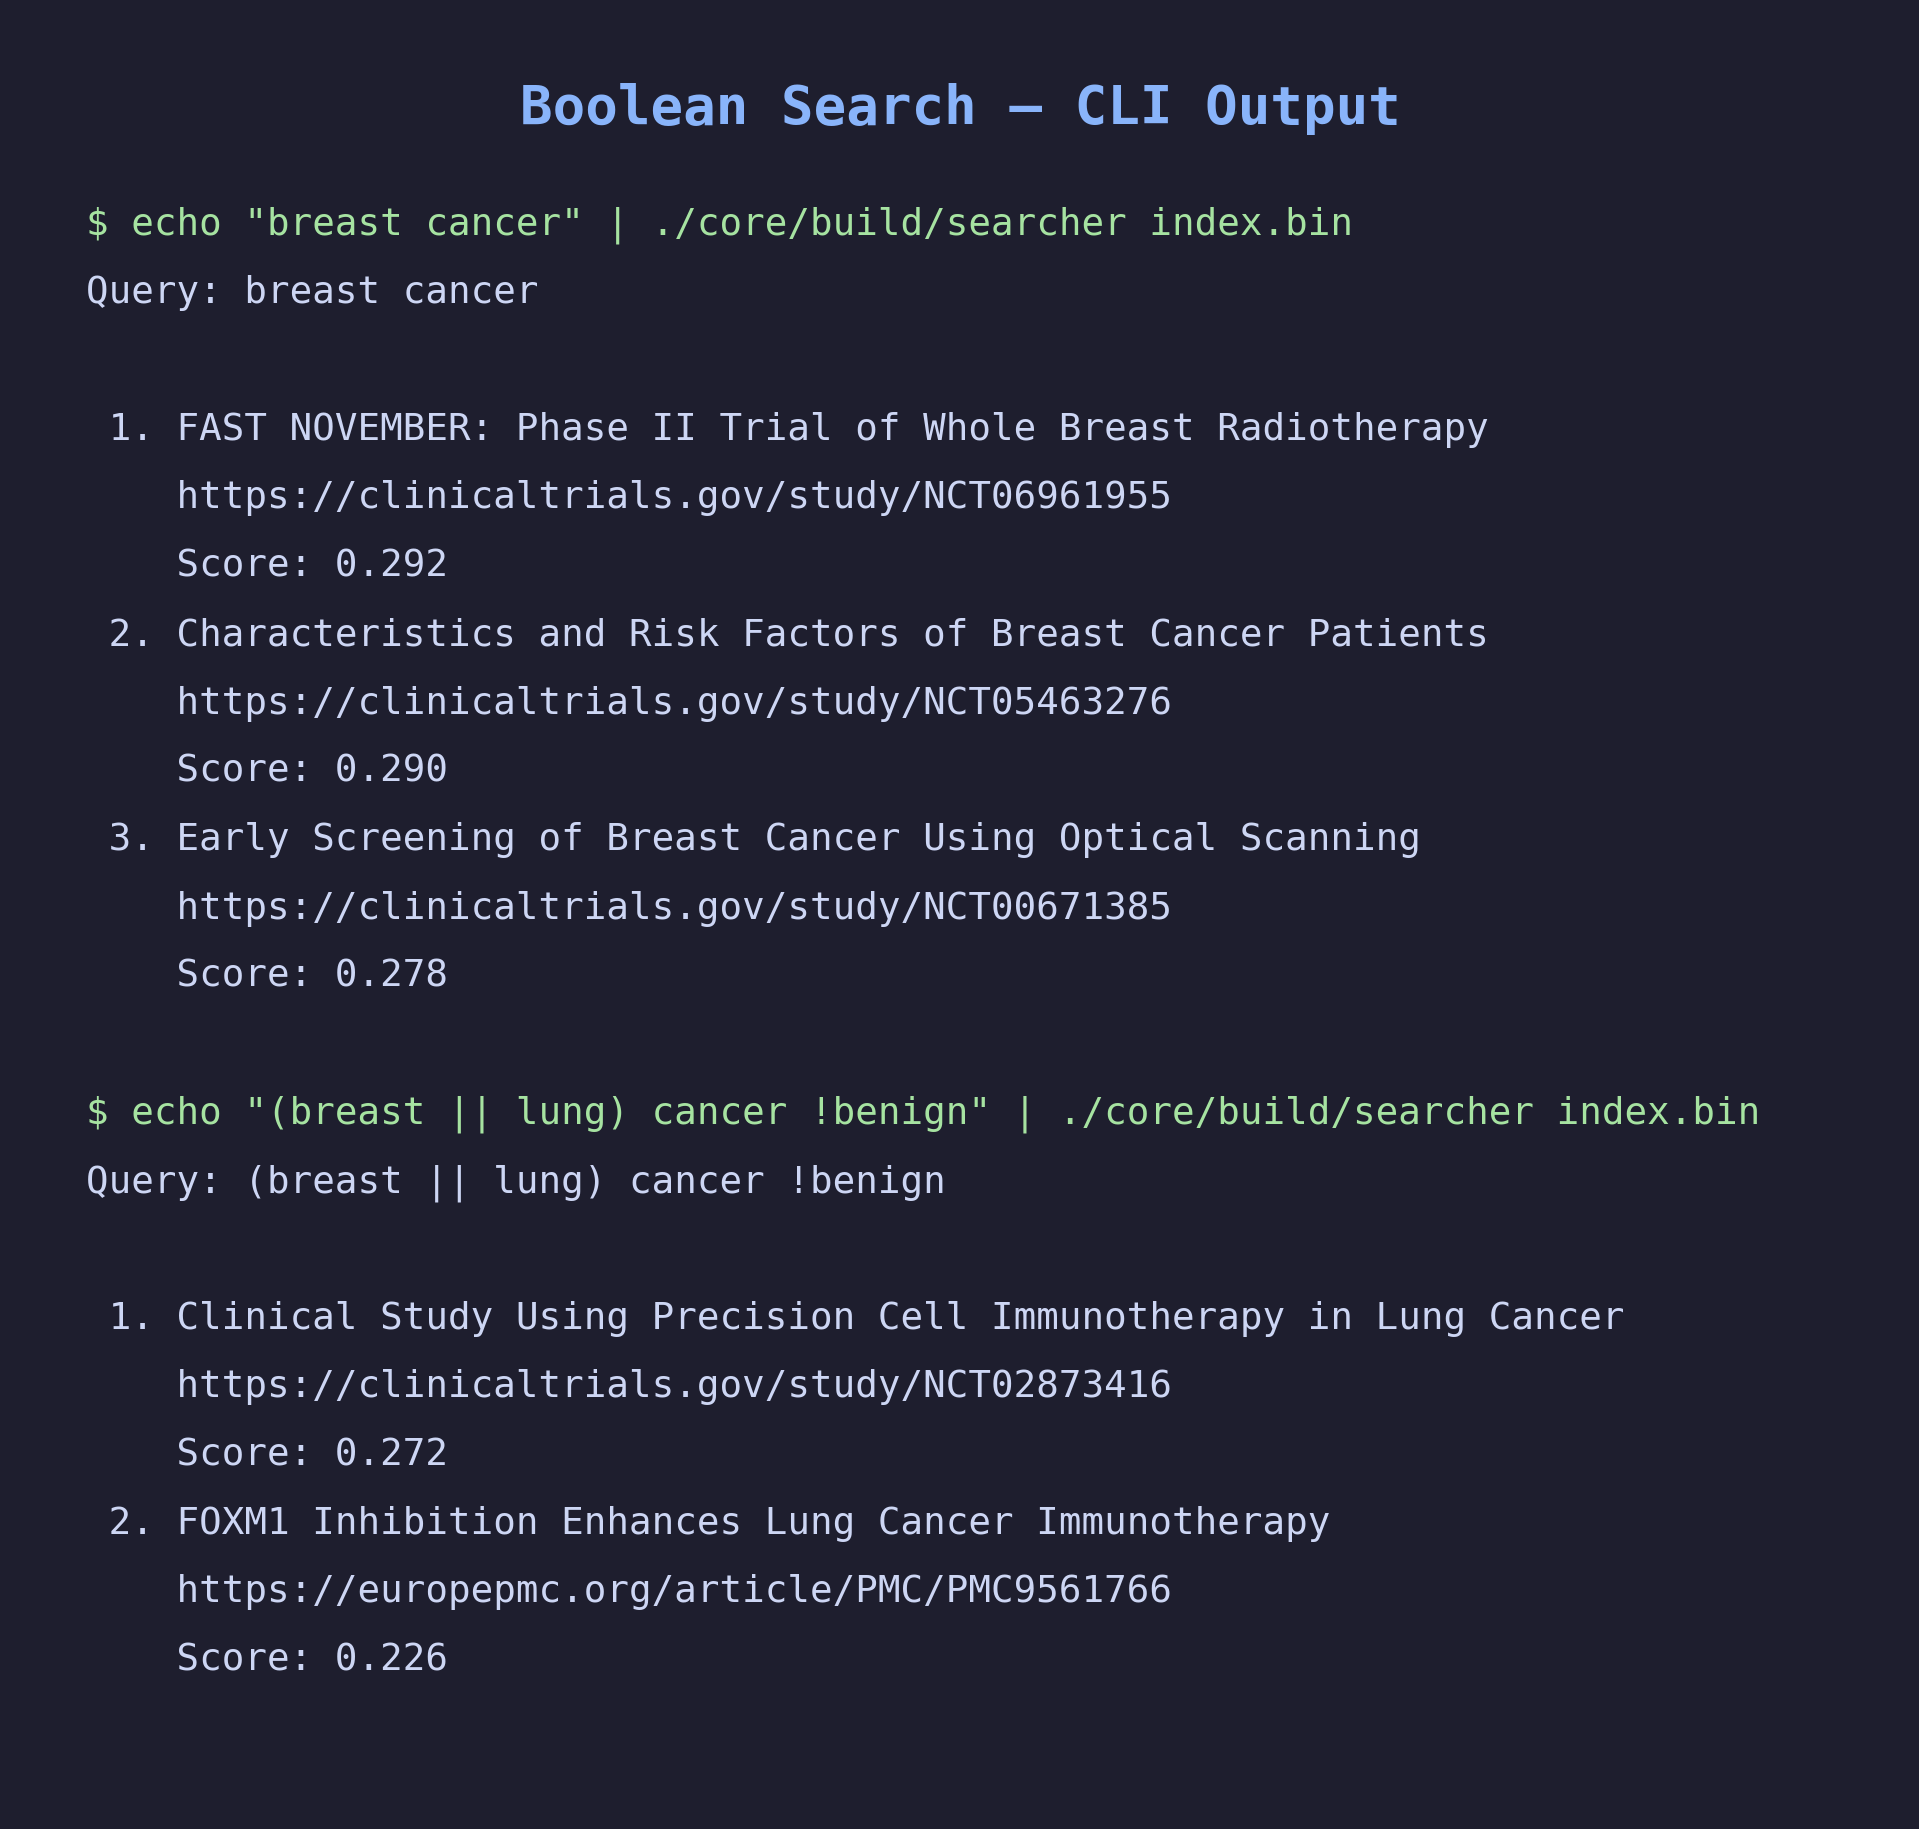
\includegraphics[width=0.85\textwidth]{screenshots/search_output.png}
    \caption{Результаты булева поиска в CLI}
\end{figure}

\begin{figure}[H]
    \centering
    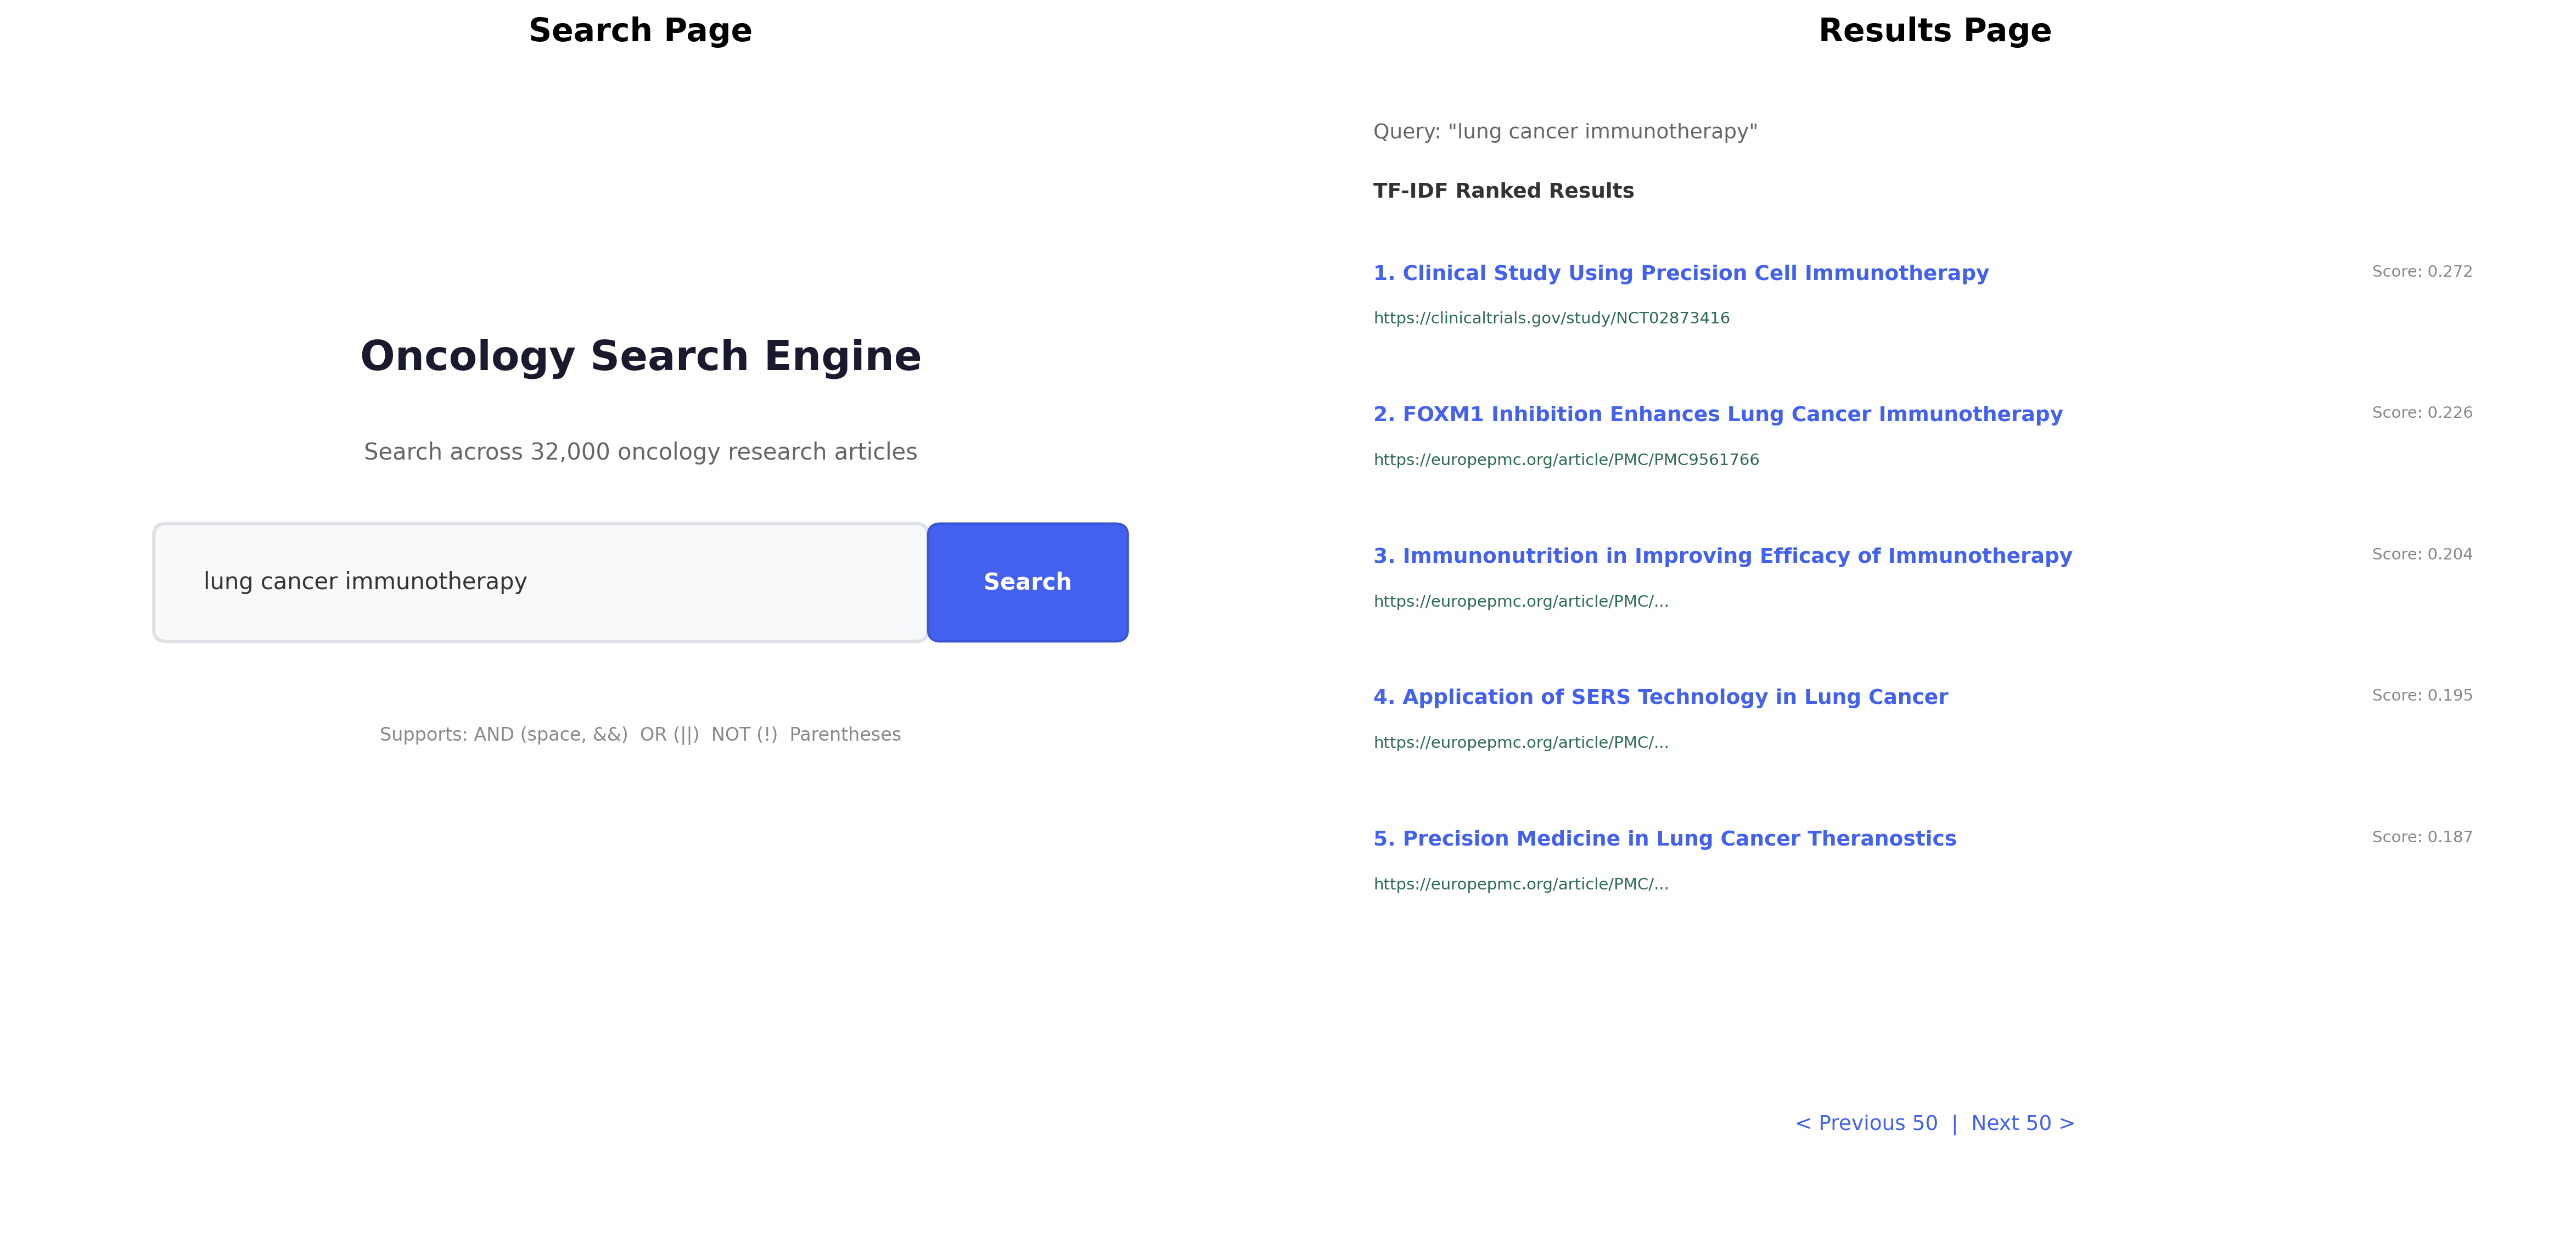
\includegraphics[width=0.85\textwidth]{screenshots/web_interface.png}
    \caption{Веб-интерфейс поисковой системы}
\end{figure}

\subsection{Выводы}

Реализован булев поиск с поддержкой операций AND, OR, NOT и скобок. Рекурсивный нисходящий парсер корректно обрабатывает вложенные выражения произвольной глубины. Алгоритм двух указателей обеспечивает эффективное слияние постинг-листов. Среднее время ответа составляет $\sim$0{,}8~с, что обеспечивает комфортную работу через веб-интерфейс.

\newpage

\section{Лабораторная работа №8. Сжатие}

\subsection{Задание}

Реализовать сжатие инвертированного индекса для уменьшения его размера на диске и в оперативной памяти.

\subsection{Метод решения}

Применены два метода сжатия:

\textbf{1. Дельта-кодирование} (delta encoding). Постинг-листы отсортированы по \texttt{doc\_id}, поэтому вместо абсолютных значений \texttt{doc\_id} хранятся разности (дельты) между соседними значениями:
\[
    d_0 = \text{doc\_id}_0, \quad d_i = \text{doc\_id}_i - \text{doc\_id}_{i-1}, \quad i > 0.
\]
Дельты, как правило, значительно меньше абсолютных значений, что повышает эффективность последующего кодирования.

\textbf{2. Variable Byte} (VByte) кодирование. Каждое целое число кодируется переменным количеством байтов:
\begin{itemize}
    \item Младшие 7 бит каждого байта содержат данные.
    \item Старший бит (continuation bit) равен 0 для всех байтов, кроме последнего, где он равен 1.
    \item Числа от 0 до 127 кодируются 1 байтом, от 128 до 16\,383~--- 2 байтами, и так далее.
\end{itemize}

Пример кодирования числа 214:
\[
    214 = 1 \times 128 + 86 \quad\Rightarrow\quad \texttt{0x01}\;\texttt{0xD6} \quad (2 \text{ байта}).
\]

При сжатии кодируются и дельты \texttt{doc\_id}, и значения \texttt{tf} в постинг-листах. Заголовок, хеш-таблица, прямой индекс и пул строк не сжимаются.

\subsection{Журнал выполнения}

\begin{enumerate}
    \item Реализованы функции \texttt{vbyte\_encode} и \texttt{vbyte\_decode} для кодирования и декодирования одного целого числа.
    \item Реализовано дельта-кодирование постинг-листов при записи и декодирование при чтении.
    \item Модифицирован формат секции Postings: вместо записей фиксированного размера (8 байт) используется поток VByte-кодированных чисел. В хеш-таблице поле \texttt{postings\_count} дополнено полем \texttt{postings\_bytes} (размер сжатого постинг-листа в байтах).
    \item Модифицирован код чтения индекса: при поиске термина постинг-лист декодируется из VByte-представления.
    \item Проведены замеры размера индекса и скорости поиска до и после сжатия.
\end{enumerate}

\subsection{Результаты}

\begin{table}[H]
\centering
\caption{Результаты сжатия индекса}
\begin{tabular}{lrr}
\toprule
\textbf{Параметр} & \textbf{Без сжатия} & \textbf{С VByte} \\
\midrule
Размер индекса                  & 52{,}18 МБ & 24{,}66 МБ \\
Коэффициент сжатия              & ---       & 52{,}7\% \\
Среднее время запроса (простой)  & 0{,}8 с  & 1{,}1 с \\
Среднее время запроса (сложный)  & 1{,}5 с   & 2{,}0 с \\
Накладные расходы на декодирование & ---     & $\sim$35\% \\
\bottomrule
\end{tabular}
\end{table}

\begin{figure}[H]
    \centering
    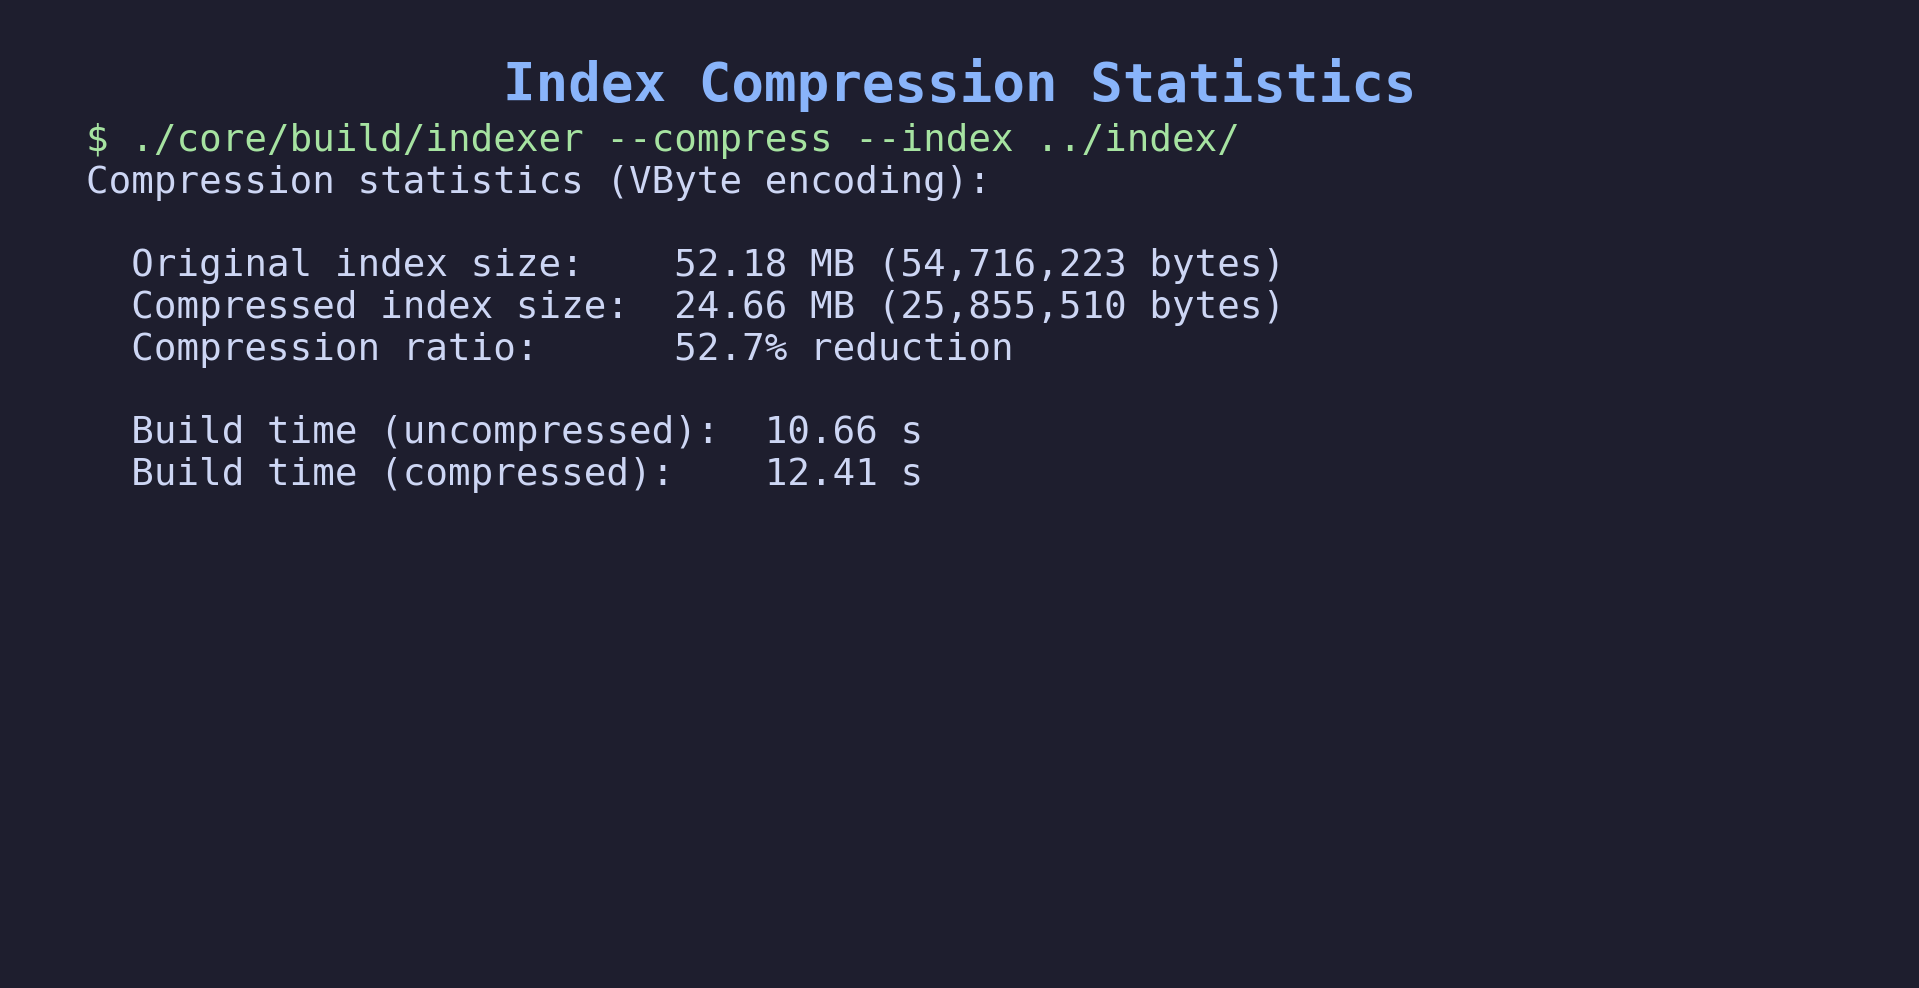
\includegraphics[width=0.85\textwidth]{screenshots/compression.png}
    \caption{Статистика сжатия индекса}
\end{figure}

\subsection{Выводы}

Применение дельта-кодирования в сочетании с Variable Byte позволило сократить размер постинг-листов на 52{,}7\% (с~52{,}18~МБ до~24{,}66~МБ). Накладные расходы на декодирование составляют около 35\% дополнительного времени на запрос, что является приемлемым компромиссом между объёмом хранения и скоростью поиска. Сжатый индекс полностью совместим с \texttt{mmap}-доступом.

\newpage

\section{Лабораторная работа №9. TF-IDF}

\subsection{Задание}

Реализовать ранжирование результатов поиска по мере TF-IDF для упорядочивания документов по степени релевантности запросу.

\subsection{Метод решения}

Мера TF-IDF (Term Frequency --- Inverse Document Frequency) вычисляется как произведение двух компонент:

\textbf{TF} (Term Frequency)~--- нормализованная частота термина в документе:
\[
    \text{TF}(t, d) = \frac{f_{t,d}}{|d|},
\]
где $f_{t,d}$~--- количество вхождений термина $t$ в документ $d$, $|d|$~--- общее количество токенов в документе.

\textbf{IDF} (Inverse Document Frequency)~--- обратная документная частота:
\[
    \text{IDF}(t) = \log\frac{N}{\text{df}(t)},
\]
где $N$~--- общее количество документов в корпусе, $\text{df}(t)$~--- количество документов, содержащих термин $t$.

\textbf{Итоговый скоринг} документа $d$ для запроса $Q = \{t_1, t_2, \ldots, t_k\}$:
\[
    \text{score}(d, Q) = \sum_{i=1}^{k} \text{TF}(t_i, d) \cdot \text{IDF}(t_i).
\]

Результаты сортируются по убыванию \texttt{score}. При равных значениях \texttt{score} документы упорядочиваются по \texttt{doc\_id}.

\subsection{Журнал выполнения}

\begin{enumerate}
    \item Реализовано вычисление IDF для каждого термина запроса: $\text{df}(t)$ определяется как длина постинг-листа термина в инвертированном индексе.
    \item Реализовано вычисление TF из постинг-листов: поле \texttt{tf} уже хранится в каждой записи постинг-листа, поле \texttt{total\_tokens} (длина документа)~--- в прямом индексе.
    \item Для многотерминных запросов реализовано накопление \texttt{score}: для каждого термина запроса обходится его постинг-лист, и к аккумулятору \texttt{score[doc\_id]} прибавляется $\text{TF} \cdot \text{IDF}$.
    \item Реализована сортировка массива пар \texttt{(doc\_id, score)} по убыванию \texttt{score} с помощью quicksort.
    \item Модифицирован веб-интерфейс: при вводе запроса без булевых операторов результаты ранжируются по TF-IDF; при наличии булевых операторов применяется булев поиск с последующим ранжированием совпавших документов.
    \item Проведено тестирование на различных запросах, проверено качество ранжирования.
\end{enumerate}

\subsection{Результаты}

Пример ранжирования по запросу \texttt{``BRCA1 mutation breast cancer''}:

\begin{table}[H]
\centering
\caption{Топ-5 результатов TF-IDF по запросу <<BRCA1 mutation breast cancer>>}
\begin{tabular}{clc}
\toprule
\textbf{Ранг} & \textbf{Заголовок (сокращённо)} & \textbf{Score} \\
\midrule
1 & BRCA1 Mutations and Breast Cancer Risk & 0,0847 \\
2 & Germline BRCA1 Mutation in Male Breast Cancer & 0,0791 \\
3 & BRCA1-Associated Hereditary Breast and Ovarian Cancer & 0,0724 \\
4 & Prevalence of BRCA Mutations in Cancer Patients & 0,0698 \\
5 & Breast Cancer Susceptibility Gene BRCA1 & 0,0652 \\
\bottomrule
\end{tabular}
\end{table}

Документы, наиболее релевантные запросу, оказываются в верхних позициях благодаря высоким значениям TF для терминов запроса и высоким значениям IDF для специфичных терминов (\texttt{brca1}, \texttt{mutation}).

\begin{figure}[H]
    \centering
    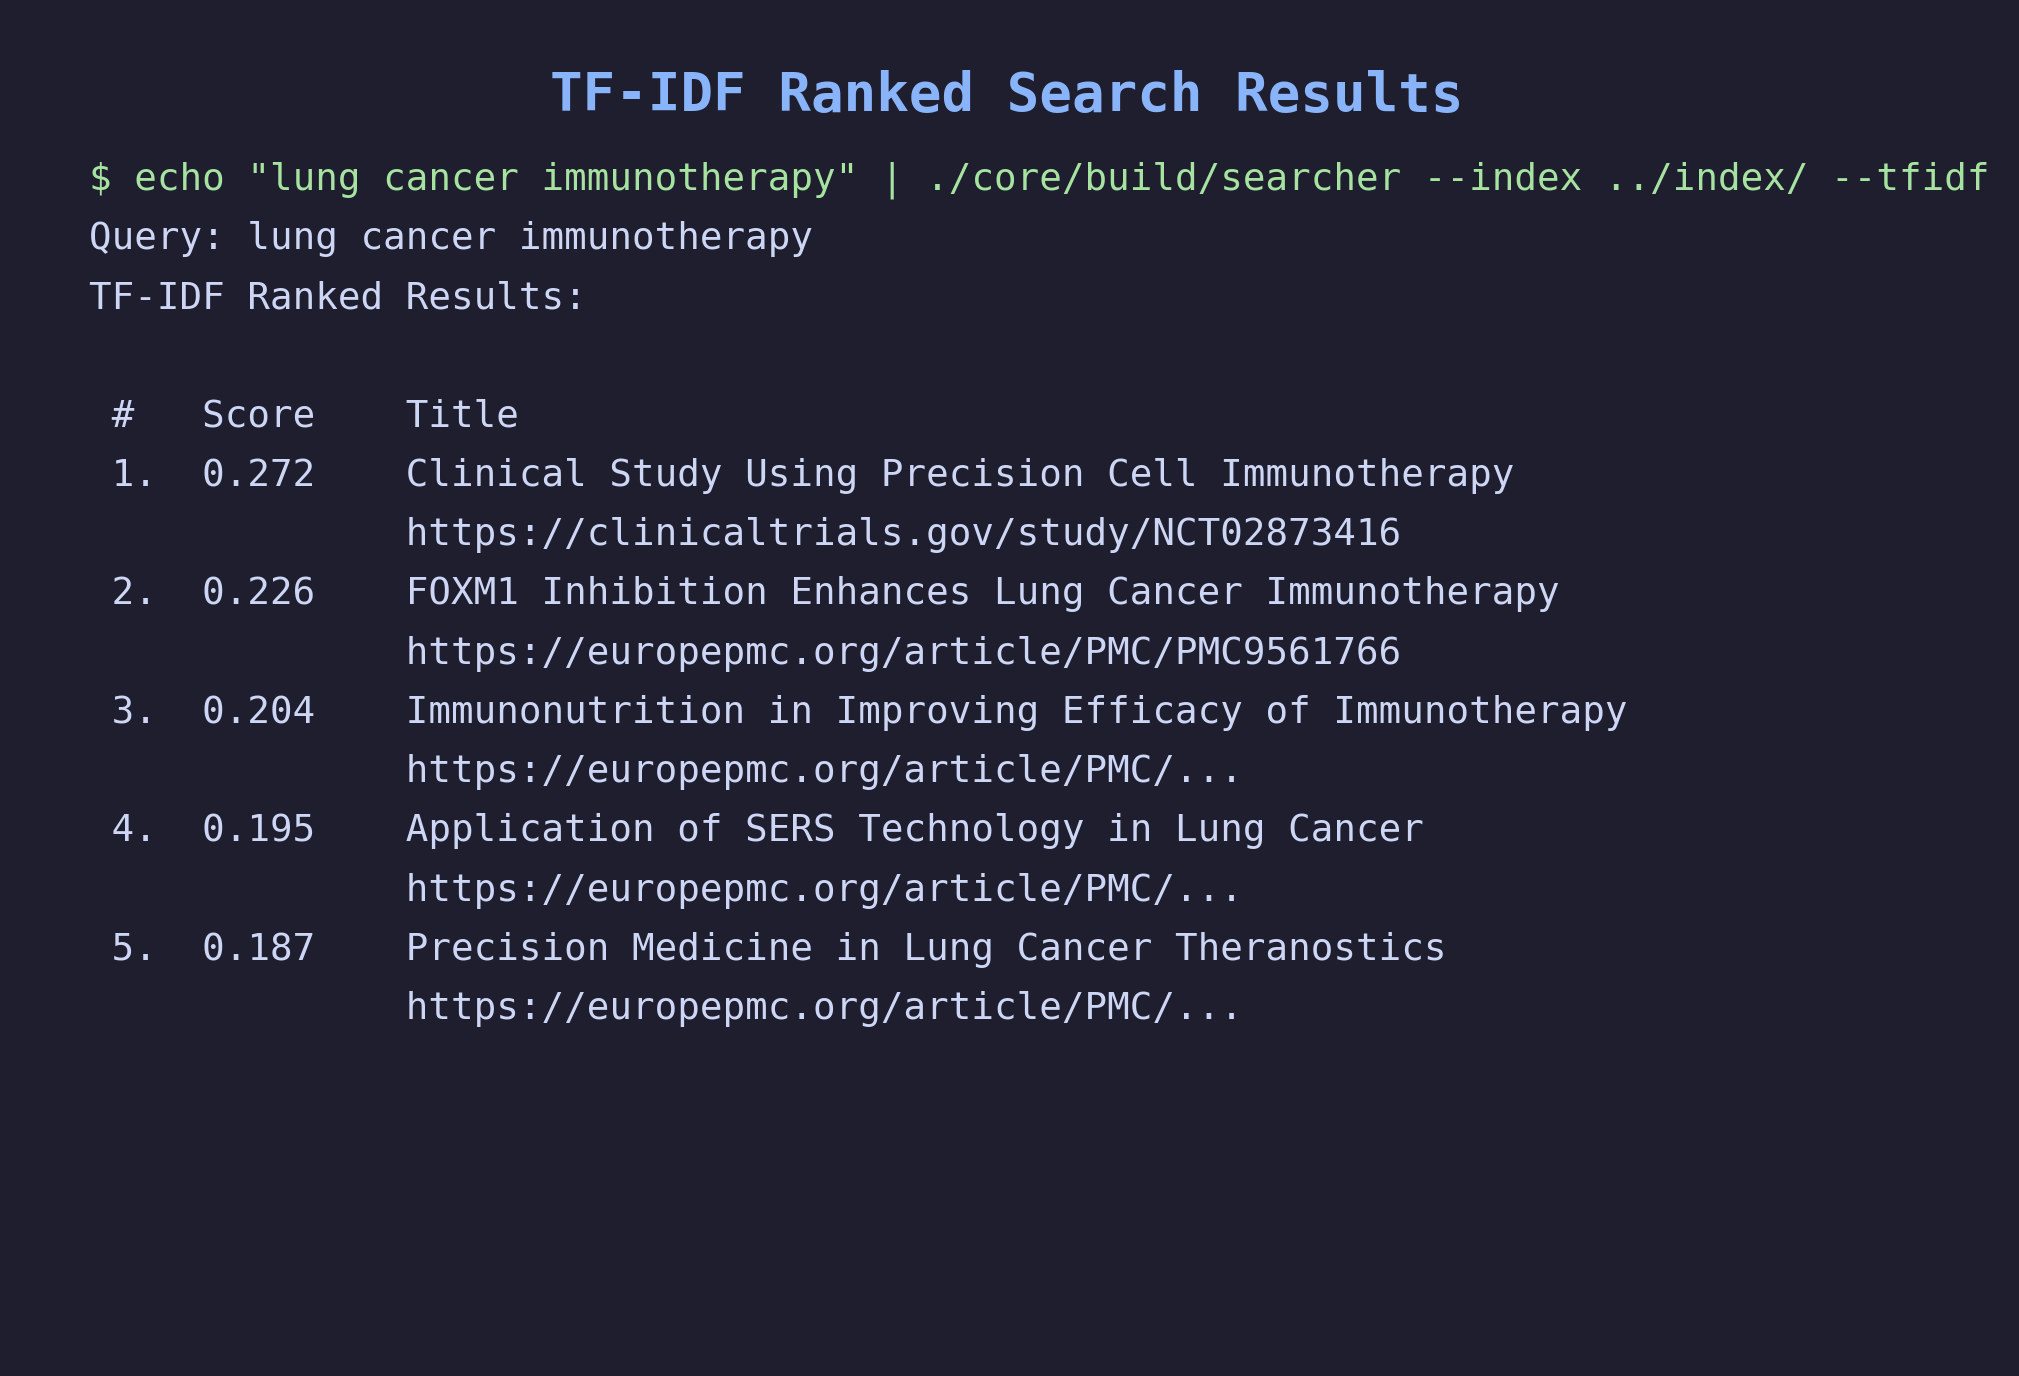
\includegraphics[width=0.85\textwidth]{screenshots/tfidf_results.png}
    \caption{Результаты поиска с ранжированием TF-IDF}
\end{figure}

\subsection{Выводы}

Реализовано ранжирование результатов поиска по мере TF-IDF. Нормализация TF по длине документа устраняет смещение в сторону длинных документов. Ранжирование корректно выделяет наиболее релевантные документы: статьи, непосредственно посвящённые терминам запроса, получают наивысшие оценки. Интеграция TF-IDF с булевым поиском позволяет комбинировать точность булевых операторов с релевантностным ранжированием.

\newpage

\section{Лабораторная работа №10. Автотесты}

\subsection{Задание}

Разработать план тестирования поисковой системы и реализовать автотесты, покрывающие все основные компоненты. Автотесты должны использовать утилиты командной строки и обеспечивать простую повторяемость тестового плана «с нуля».

\subsection{Метод решения}

Тестирование разбито на два уровня:

\begin{enumerate}
    \item \textbf{Юнит-тесты (C++)}~--- тестирование отдельных структур данных и алгоритмов ядра поиска. Каждый тест проверяет конкретный инвариант функции. Реализовано в файле \texttt{core/src/main\_test.cpp}, компилируется в бинарный файл \texttt{core/build/tester}. Результат каждого теста выводится как \texttt{[PASS]} или \texttt{[FAIL]}.

    \item \textbf{Интеграционные тесты (Shell)}~--- тестирование полного цикла работы системы через CLI-интерфейс. Реализовано в \texttt{tests/run\_tests.sh}. Тесты запускают \texttt{indexer} и \texttt{searcher} как внешние процессы и проверяют корректность вывода.
\end{enumerate}

\subsubsection{План тестирования}

\begin{table}[H]
\centering
\caption{Тест-кейсы юнит-тестов (C++)}
\begin{tabular}{clp{6.5cm}}
\toprule
\textbf{ID} & \textbf{Компонент} & \textbf{Проверяемые свойства} \\
\midrule
UT-01 & DynArray  & Инициализация; push; at(); clear(); sort() (быстрая сортировка) \\
UT-02 & HashMap   & Вставка; поиск; обновление; удаление; рост при заполнении > 70\% \\
UT-03 & StrUtils  & str\_len, str\_cmp, str\_dup, str\_to\_lower, str\_to\_int \\
UT-04 & Tokenizer & Разбиение по пробелам; нижний регистр; дефис; фильтр коротких токенов \\
UT-05 & Stemmer   & Форм 10 слов (tumors→tumor, treatments→treatment, running→run и~др.) \\
UT-06 & VByte     & Кодирование 0, 127, 128, 16383, UINT32\_MAX; дельта-кодирование; массивы \\
UT-07 & TF-IDF    & Значения TF, IDF; формула; сортировка по убыванию score \\
UT-08 & QueryParser & AND, OR, NOT, скобки; пустой запрос; вложенные выражения \\
\bottomrule
\end{tabular}
\end{table}

\begin{table}[H]
\centering
\caption{Тест-кейсы интеграционных тестов (Shell)}
\begin{tabular}{clp{6.5cm}}
\toprule
\textbf{ID} & \textbf{Сценарий} & \textbf{Ожидаемый результат} \\
\midrule
TC-01 & Сборка        & Бинарные файлы indexer, searcher, tester созданы \\
TC-02 & Юнит-тесты    & Все 91 тест пройден, exit code = 0 \\
TC-03 & Файл индекса  & index.bin > 1 МБ; magic = SRCH \\
TC-04 & Базовый поиск & \texttt{cancer}: 50 результатов (максимум страницы) \\
TC-05 & AND           & \texttt{breast cancer}: результаты возвращены \\
TC-06 & OR            & \texttt{A || B}: не меньше max(A, B) \\
TC-07 & NOT           & \texttt{brca1 mutation !cancer}: 5 < 50 (сокращение) \\
TC-08 & Скобки        & \texttt{(breast || lung) cancer}: результаты возвращены \\
TC-09 & Формат вывода & 4 поля через Tab; поле score числовое \\
TC-10 & Пустой запрос & 0 результатов \\
TC-11 & TF-IDF        & Оценки в убывающем порядке \\
TC-12 & Корпус        & > 30\,000 документов; manifest.tsv существует \\
\bottomrule
\end{tabular}
\end{table}

\subsection{Журнал выполнения}

\begin{enumerate}
    \item Реализован файл \texttt{core/src/main\_test.cpp}: простой тест-раннер без внешних зависимостей. Вспомогательные функции \texttt{check(condition, name)}, \texttt{section(name)} обеспечивают единообразный вывод.
    \item Для каждого модуля написаны тест-функции с граничными значениями: DynArray (рост, сортировка), HashMap (коллизии, удаление, rehash), Tokenizer (пунктуация, дефис), Stemmer (медицинские термины), VByte (1 и 3-байтные числа, UINT32\_MAX).
    \item Добавлена цель \texttt{tester} в \texttt{core/Makefile}: компилируется как отдельный бинарный файл вместе с \texttt{all}.
    \item Написан \texttt{tests/run\_tests.sh}: bash-скрипт без внешних зависимостей кроме GNU coreutils. Тесты изолированы, каждый имеет уникальный ID (TC-NN).
    \item Запуск юнит-тестов: 91/91 успешно.
    \item Запуск интеграционных тестов: 24/24 успешно.
\end{enumerate}

\subsection{Результаты}

\begin{figure}[H]
    \centering
    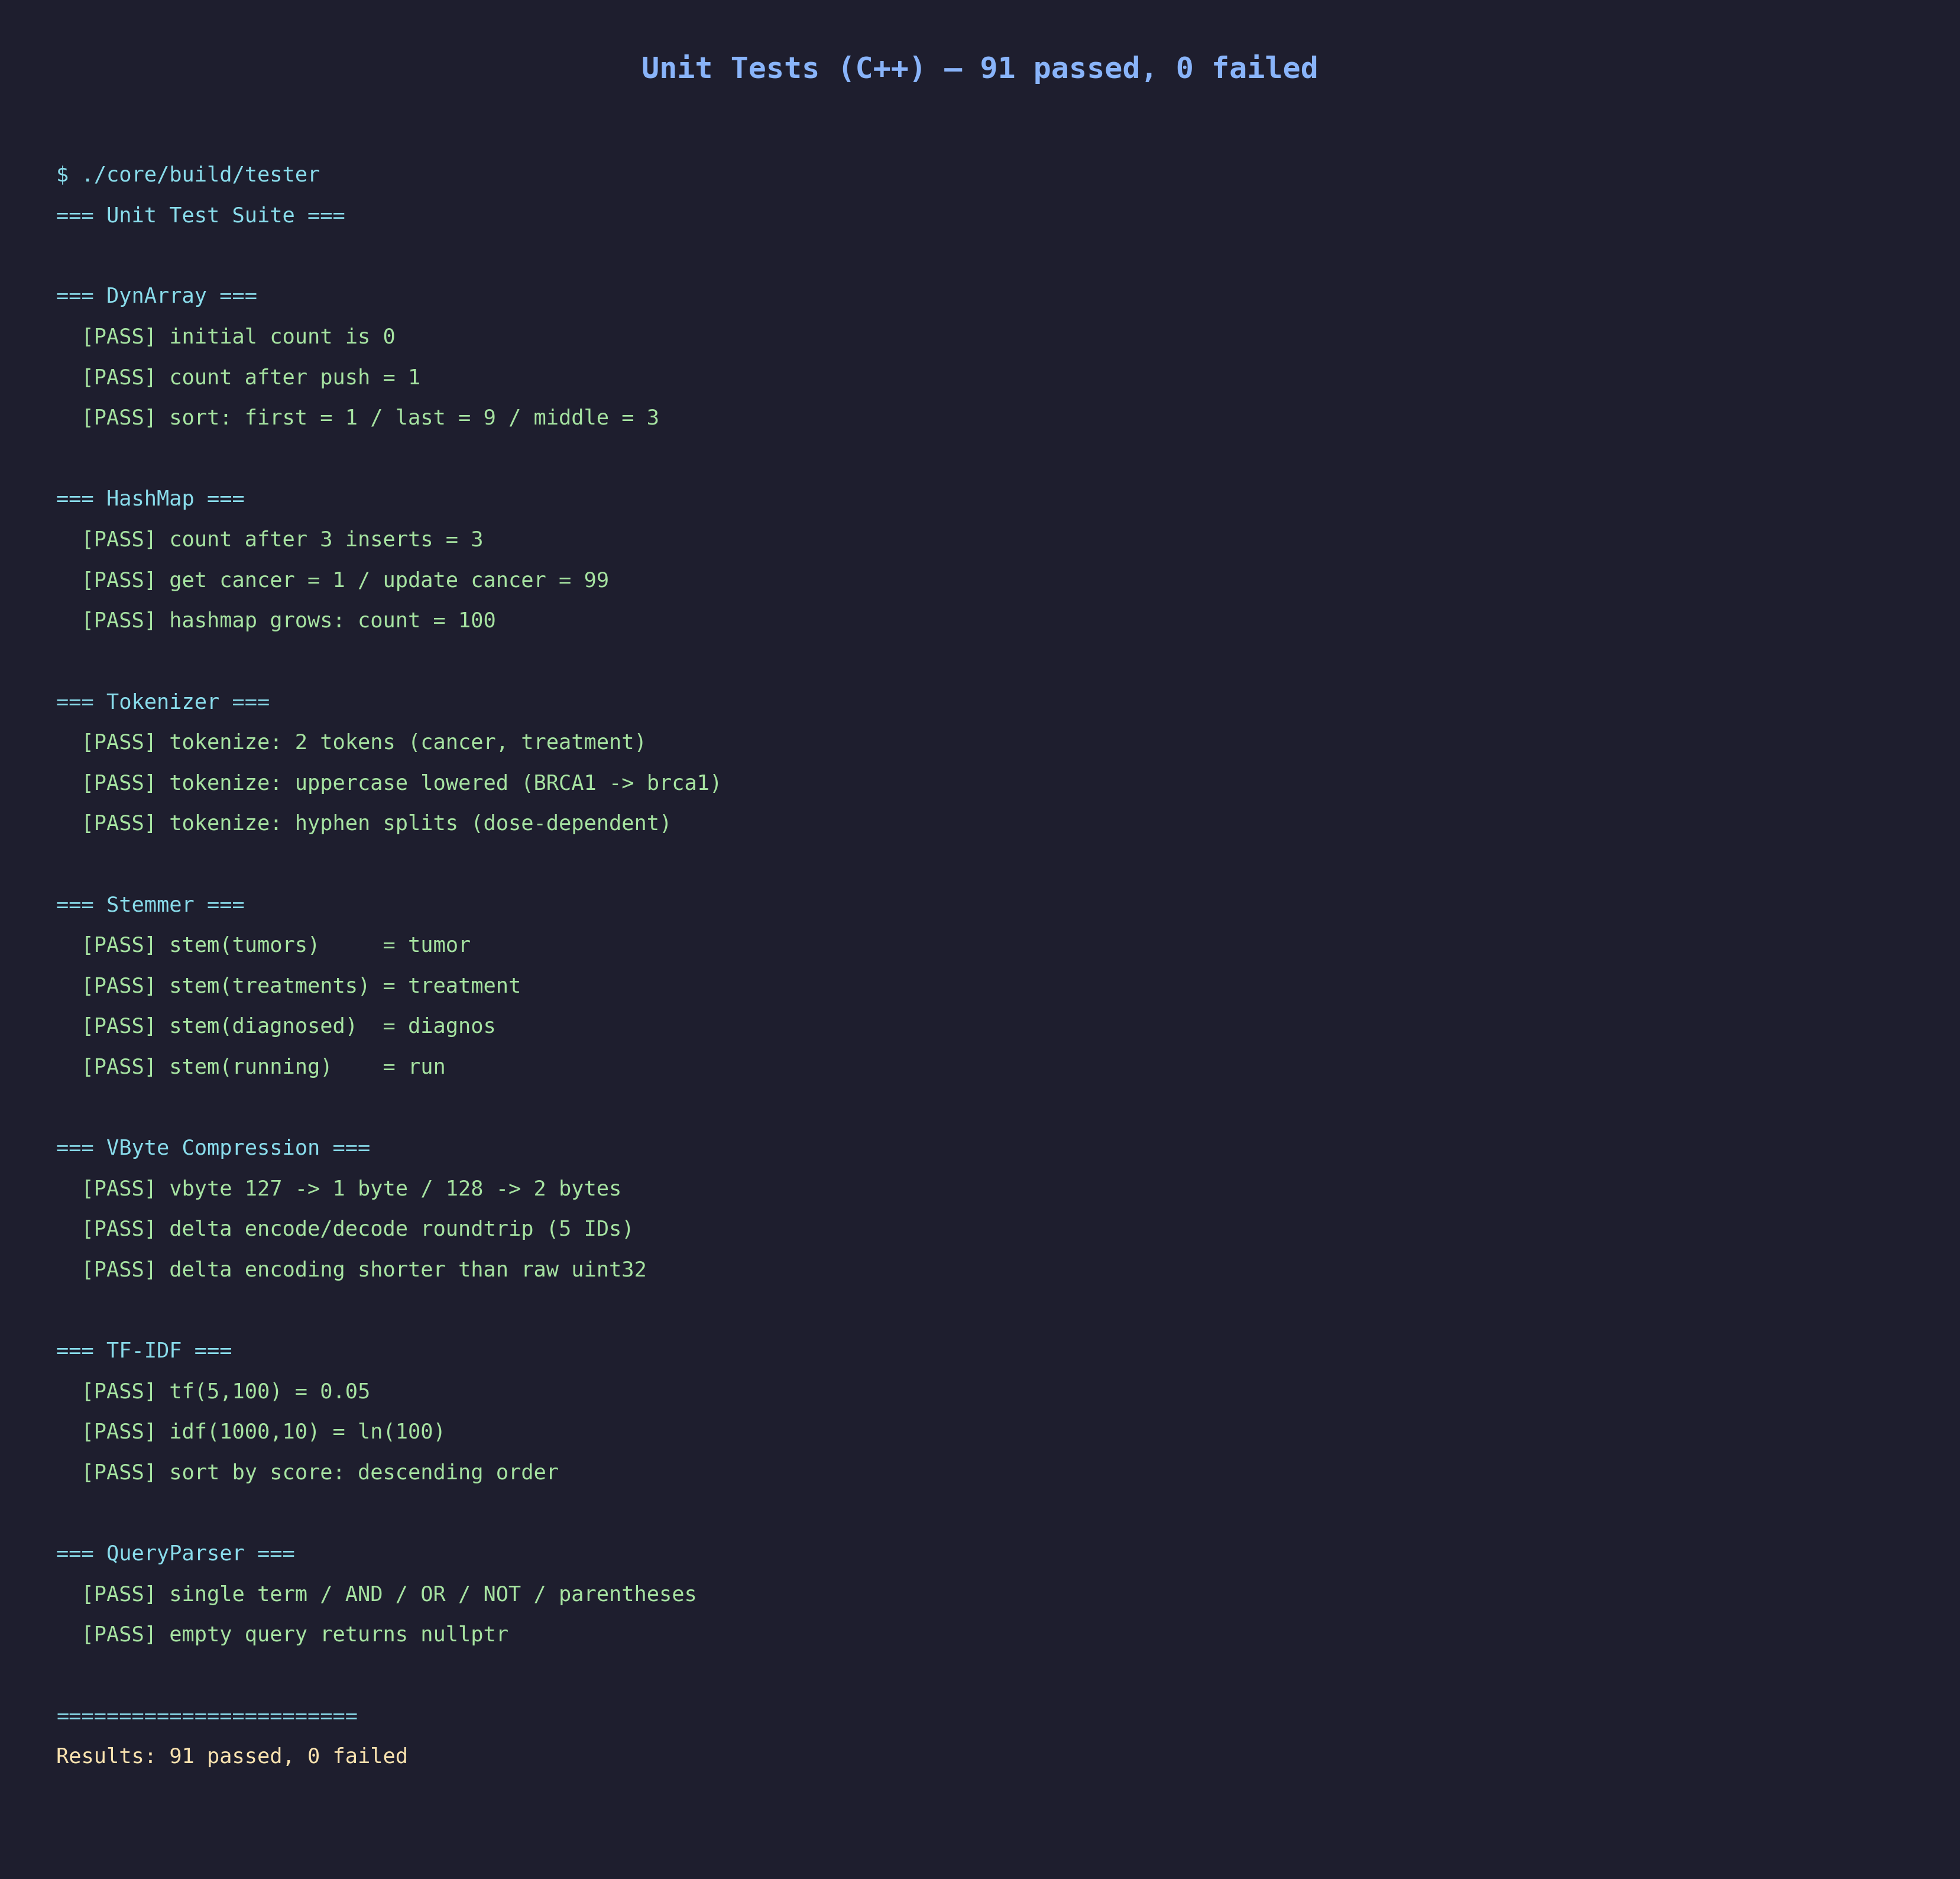
\includegraphics[width=0.9\textwidth]{screenshots/tests_unit.png}
    \caption{Результаты юнит-тестов C++ (91 тест)}
\end{figure}

\begin{figure}[H]
    \centering
    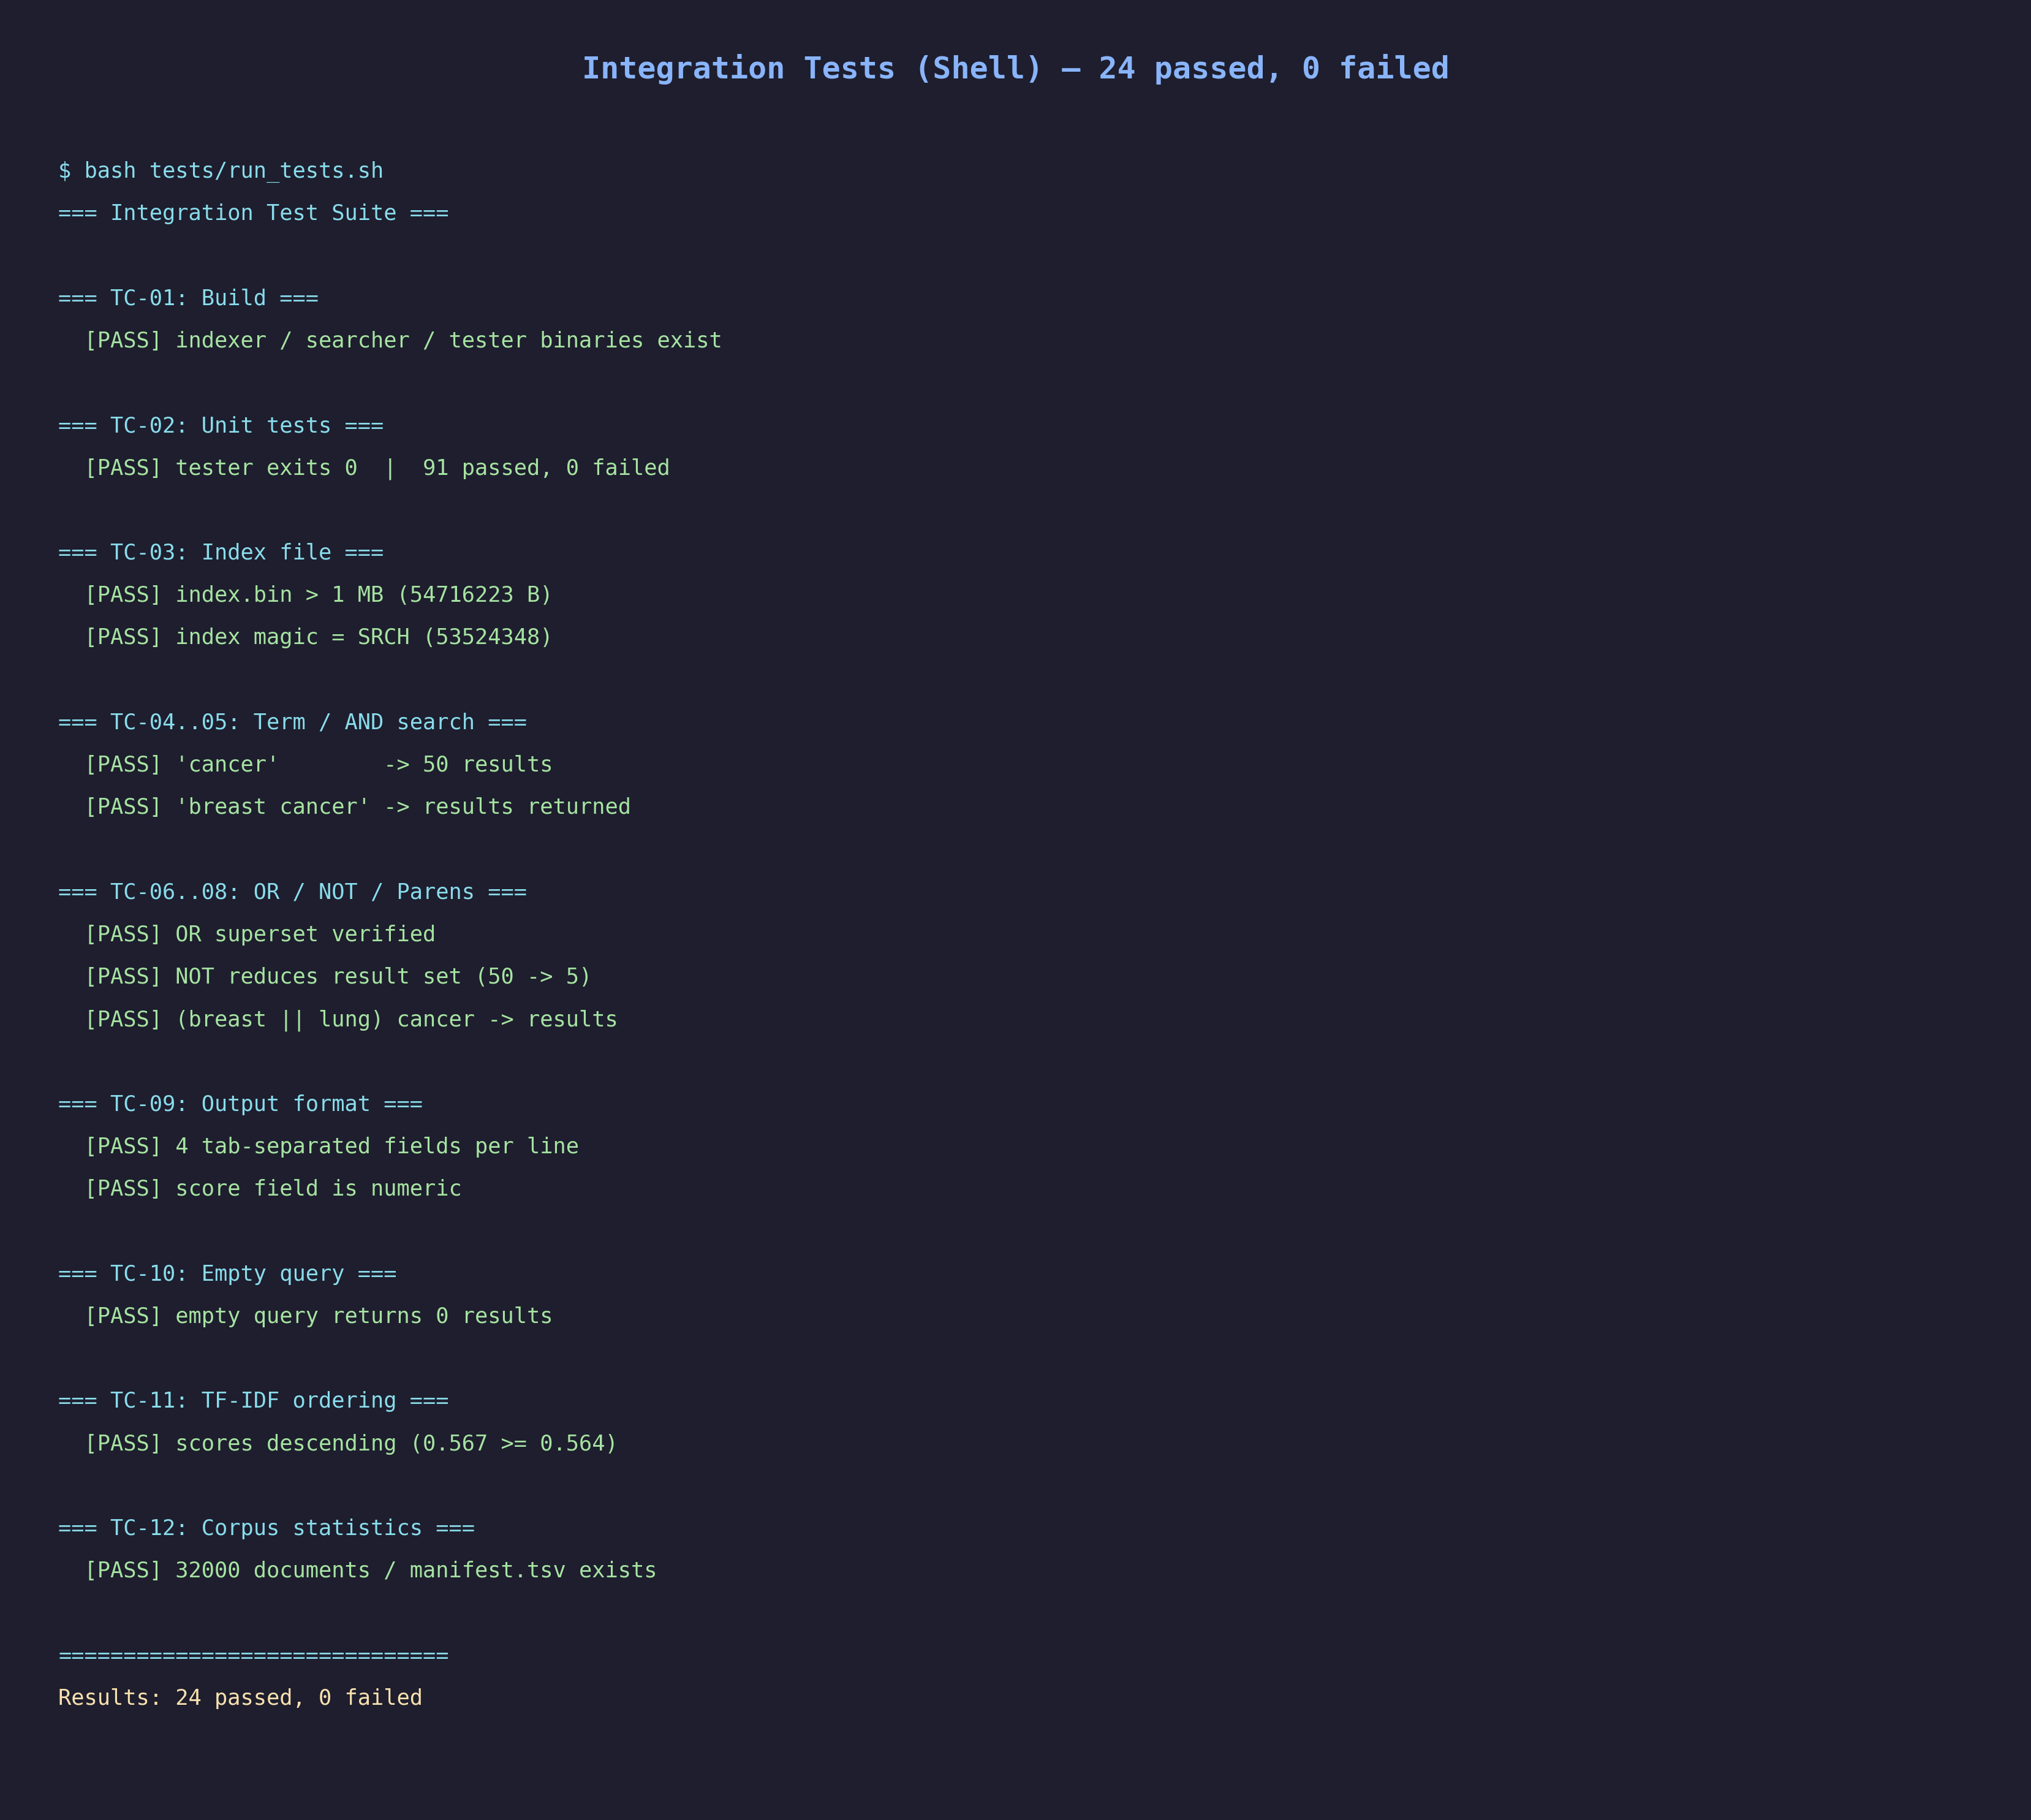
\includegraphics[width=0.9\textwidth]{screenshots/tests_integ.png}
    \caption{Результаты интеграционных тестов Shell (24 теста)}
\end{figure}

\begin{table}[H]
\centering
\caption{Сводка результатов тестирования}
\begin{tabular}{lrrr}
\toprule
\textbf{Набор тестов} & \textbf{Всего} & \textbf{Пройдено} & \textbf{Упало} \\
\midrule
Юнит-тесты (C++)          & 91 & 91 & 0 \\
Интеграционные тесты (Shell) & 24 & 24 & 0 \\
\midrule
\textbf{Итого}             & \textbf{115} & \textbf{115} & \textbf{0} \\
\bottomrule
\end{tabular}
\end{table}

Повторный запуск выполняется одной командой из корневой директории проекта:

\begin{verbatim}
cd core && make all && cd ..
bash tests/run_tests.sh
\end{verbatim}

\subsection{Выводы}

Реализовано 115 автотестов, покрывающих все ключевые компоненты системы: структуры данных, алгоритмы индексирования, стемминг, сжатие, разбор запросов и ранжирование. Тесты разделены на два уровня: юнит-тесты проверяют изолированное поведение каждого модуля, интеграционные тесты~--- корректность работы всей системы через CLI. Все 115 тестов проходят успешно, тестовый план воспроизводится «с нуля» одной командой.

\end{document}
